\subsection{Shape analysis}
\label{subsec:shape}

A shape analysis is performed in the $\met$ distribution. \textcolor{red}{The plots in this section were made earlier for top tagging which includes the boosted category. We choose not to pursue this category for the December deadline; this section will be updated shortly} Compared with the cut-and-count analysis for the inclusive selections, the shape analysis improves the sensitivity by about $25\%$ in each the hadronic and the semileptonic channel. The limits on the cross section ratio and $M_*$ are shown in Fig.~\ref{fig:rlimits_incl_shape} and Fig.~\ref{fig:mstarlimits_incl_shape}, respectively.

\begin{figure}[htbp]
\begin{center}
  \subfigure[Hadronic]{\label{subfig:hadronic_incl_shape}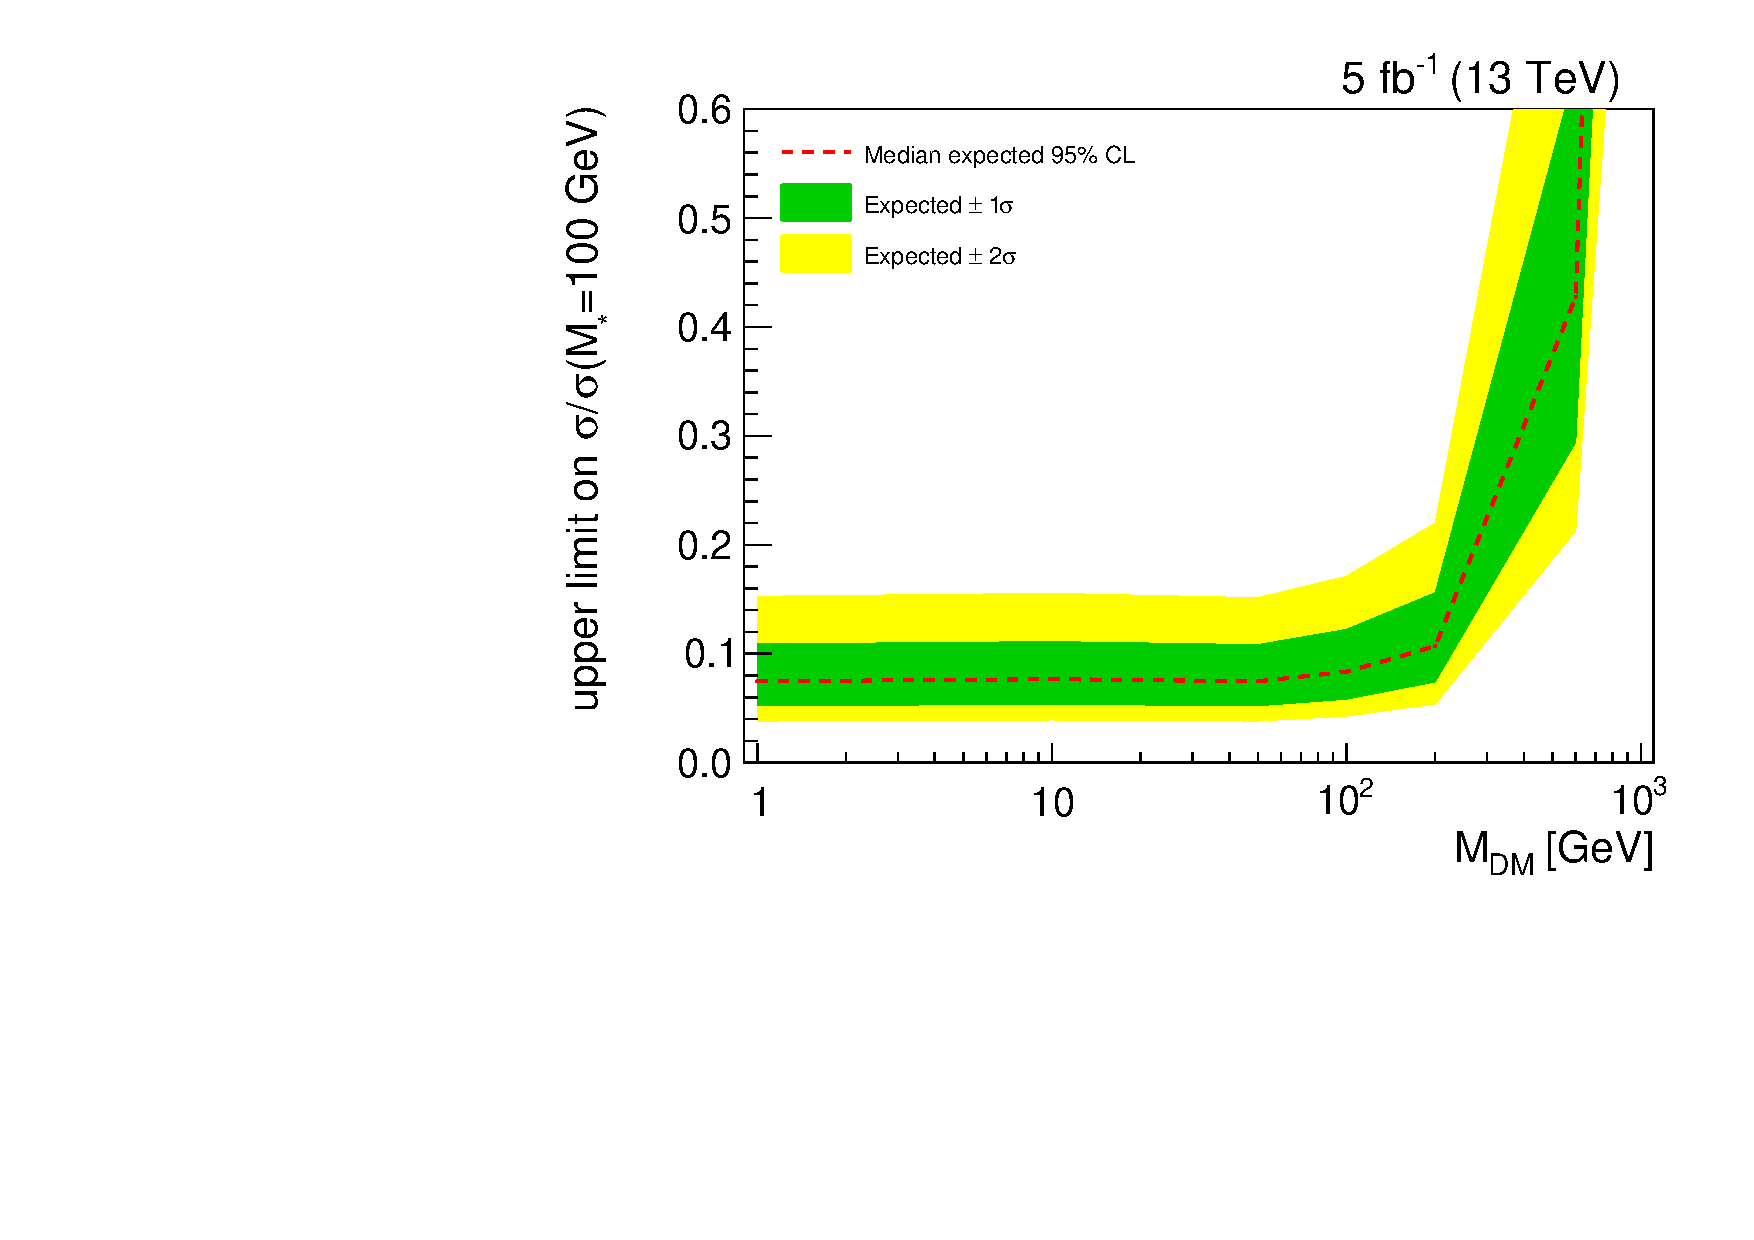
\includegraphics[width=0.32\textwidth]{figures/rLimit_hadronic_incl_shape.pdf}}
  \subfigure[Semileptonic]{\label{subfig:semilept_incl_shape}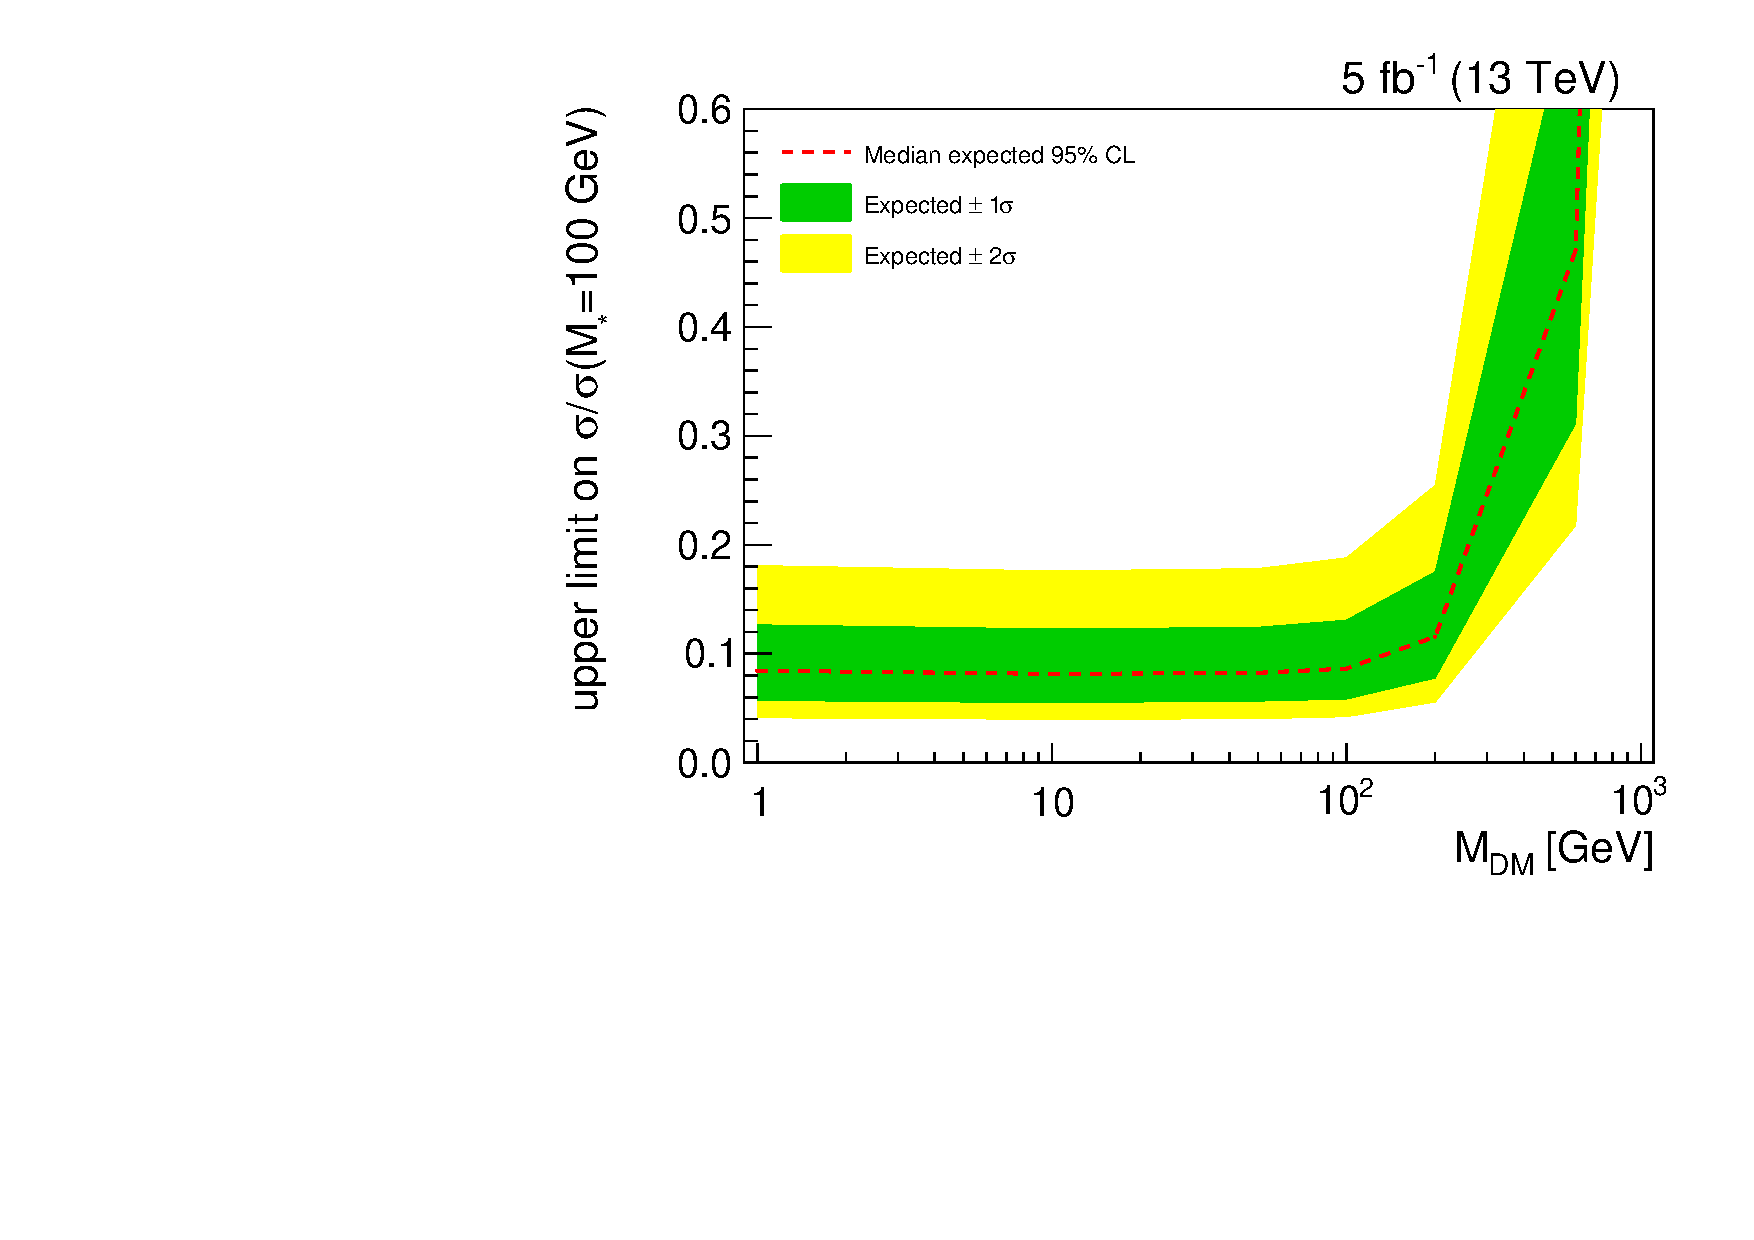
\includegraphics[width=0.32\textwidth]{figures/rLimit_semilept_incl_shape.pdf}}
  \subfigure[Combined]{\label{subfig:combined_incl_shape}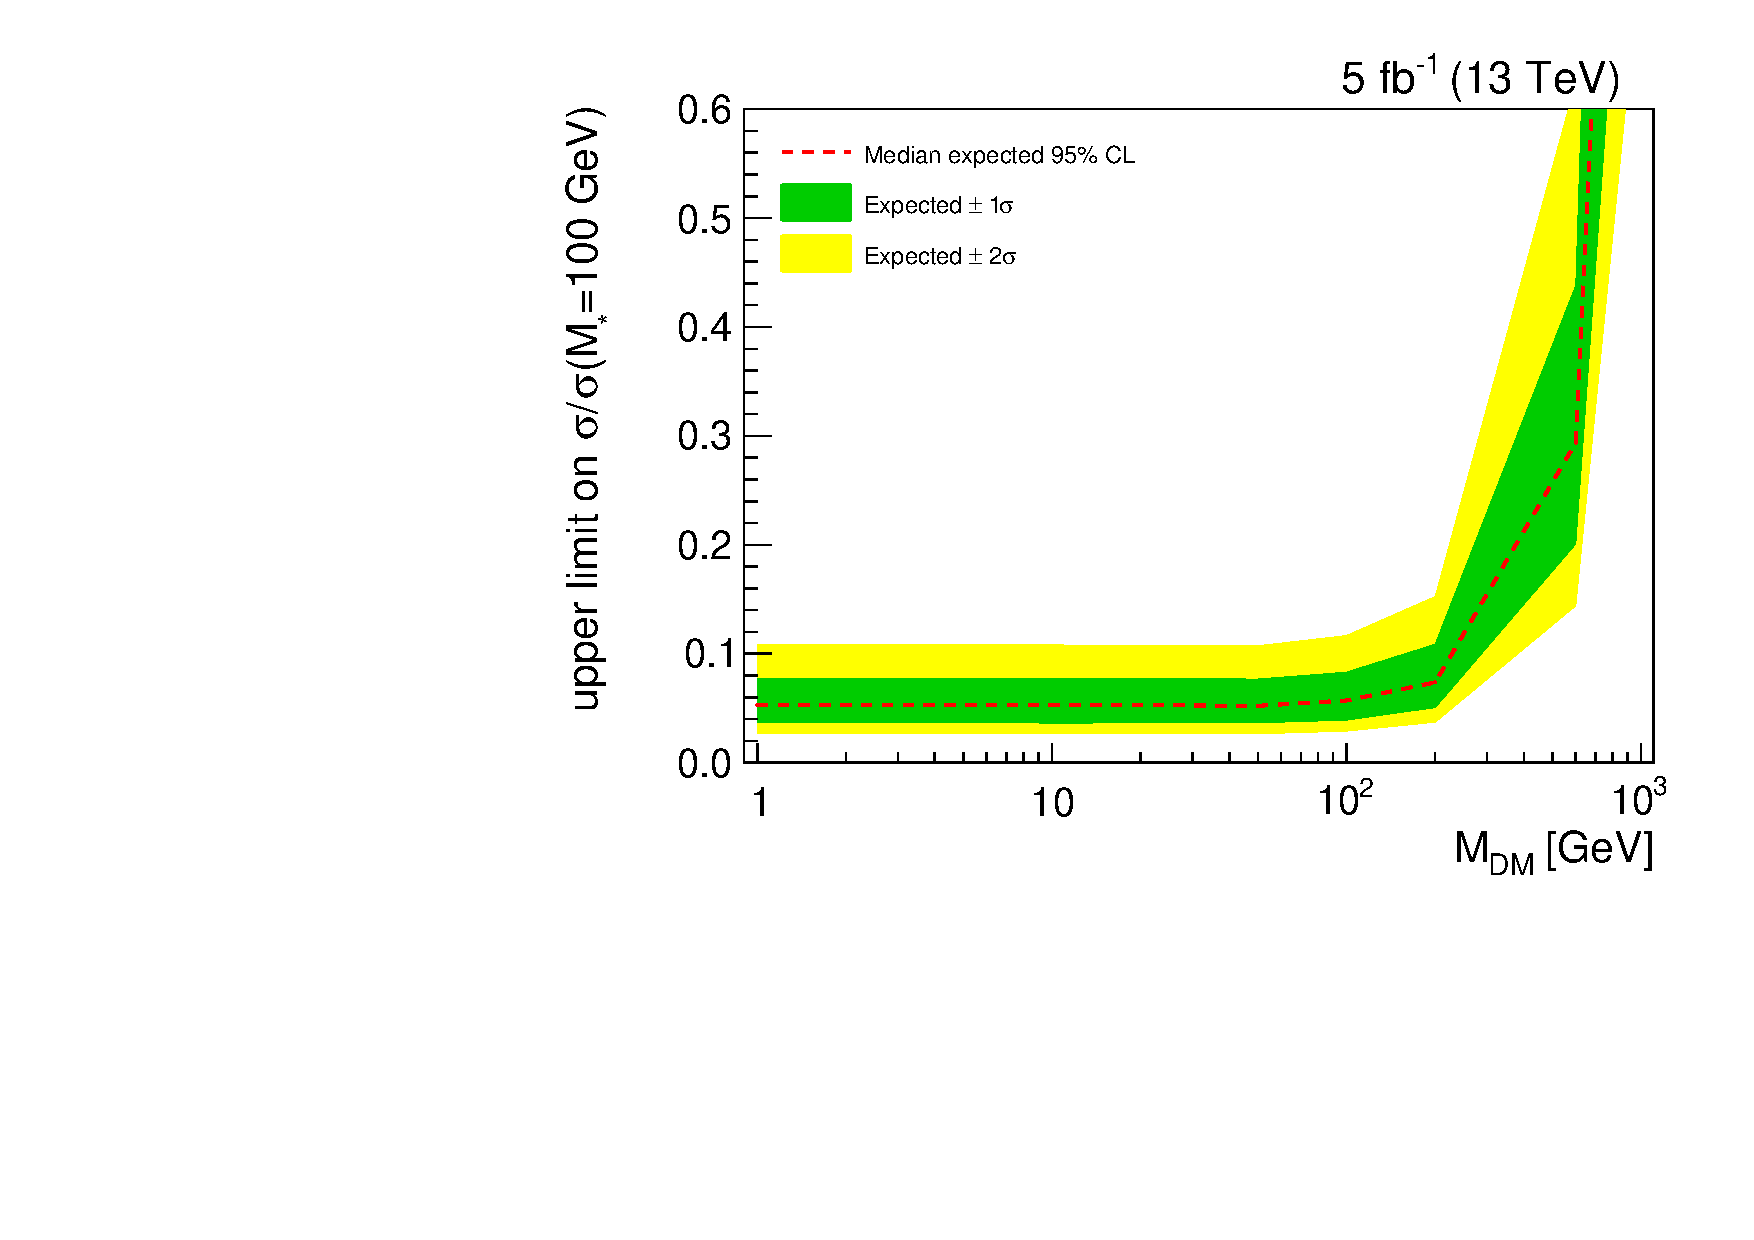
\includegraphics[width=0.32\textwidth]{figures/rLimit_incl_shape.pdf}}
  \caption{Expected upper limits on the cross section ratio relative to $M_*=100\:\GeV$ for the inclusive selections: \subref{subfig:hadronic_incl_shape} hadronic channel, \subref{subfig:semilept_incl_shape} semileptonic channel, and \subref{subfig:combined_incl_shape} combination of both channels.}
  \label{fig:rlimits_incl_shape}
\end{center}
\end{figure}

\begin{table}[!ht]
\centering
\begin{tabular}{|r|c|c|c|}
\hline
  $M_\chi$ $(\GeV)$ & Median & $\left[-1\sigma\, +1\sigma\right]$ & $\left[-2\sigma\, +2\sigma\right]$ \\
\hline
  $1$               & $0.0747$ & $\left[0.0522\, 0.1090\right]$ & $\left[0.0382\, 0.1528\right]$ \\
  $10$              & $0.0767$ & $\left[0.0536\, 0.1112\right]$ & $\left[0.0392\, 0.1555\right]$ \\
  $50$              & $0.0747$ & $\left[0.0522\, 0.1084\right]$ & $\left[0.0382\, 0.1515\right]$ \\
  $100$             & $0.0835$ & $\left[0.0583\, 0.1224\right]$ & $\left[0.0427\, 0.1712\right]$ \\
  $200$             & $0.1069$ & $\left[0.0742\, 0.1560\right]$ & $\left[0.0539\, 0.2201\right]$ \\
  $600$             & $0.4277$ & $\left[0.2944\, 0.6374\right]$ & $\left[0.2130\, 0.9043\right]$ \\
  $1000$            & $2.2109$ & $\left[1.4913\, 3.3125\right]$ & $\left[1.0666\, 4.7647\right]$ \\
\hline
\end{tabular}
\caption{Expected upper limits on the cross section ratio relative to $M_*=100\:\GeV$ for inclusive selection in the hadronic channel.}
\label{tab:rLimits_hadronic_shape}
\end{table}

\begin{table}[!ht]
\centering
\begin{tabular}{|r|c|c|c|}
\hline
  $M_\chi$ $(\GeV)$ & Median & $\left[-1\sigma\, +1\sigma\right]$ & $\left[-2\sigma\, +2\sigma\right]$ \\
\hline
  $1$               & $0.0845$ & $\left[0.0571\, 0.1266\right]$ & $\left[0.0412\, 0.1810\right]$ \\
  $10$              & $0.0815$ & $\left[0.0551\, 0.1228\right]$ & $\left[0.0398\, 0.1761\right]$ \\
  $50$              & $0.0825$ & $\left[0.0565\, 0.1243\right]$ & $\left[0.0403\, 0.1782\right]$ \\
  $100$             & $0.0864$ & $\left[0.0584\, 0.1309\right]$ & $\left[0.0422\, 0.1881\right]$ \\
  $200$             & $0.1157$ & $\left[0.0777\, 0.1752\right]$ & $\left[0.0556\, 0.2546\right]$ \\
  $600$             & $0.4707$ & $\left[0.3117\, 0.7202\right]$ & $\left[0.2179\, 1.0563\right]$ \\
  $1000$            & $2.5859$ & $\left[1.6942\, 4.0187\right]$ & $\left[1.1768\, 5.9561\right]$ \\
\hline
\end{tabular}
\caption{Expected upper limits on the cross section ratio relative to $M_*=100\:\GeV$ for inclusive selection in the semileptonic channel.}
\label{tab:rLimits_semilept_shape}
\end{table}

\begin{table}[!ht]
\centering
\begin{tabular}{|r|c|c|c|}
\hline
  $M_\chi$ $(\GeV)$ & Median & $\left[-1\sigma\, +1\sigma\right]$ & $\left[-2\sigma\, +2\sigma\right]$ \\
\hline
  $1$               & $0.0532$ & $\left[0.0373\, 0.0774\right]$ & $\left[0.0270\, 0.1081\right]$ \\
  $10$              & $0.0532$ & $\left[0.0364\, 0.0774\right]$ & $\left[0.0270\, 0.1081\right]$ \\
  $50$              & $0.0522$ & $\left[0.0366\, 0.0768\right]$ & $\left[0.0265\, 0.1073\right]$ \\
  $100$             & $0.0571$ & $\left[0.0391\, 0.0831\right]$ & $\left[0.0290\, 0.1167\right]$ \\
  $200$             & $0.0737$ & $\left[0.0506\, 0.1087\right]$ & $\left[0.0372\, 0.1525\right]$ \\
  $600$             & $0.2939$ & $\left[0.2009\, 0.4381\right]$ & $\left[0.1441\, 0.6250\right]$ \\
  $1000$            & $1.5430$ & $\left[1.0407\, 2.3118\right]$ & $\left[0.7444\, 3.3252\right]$ \\
\hline
\end{tabular}
\caption{Expected upper limits on the cross section ratio relative to $M_*=100\:\GeV$ for combined hadronic and semileptonic channel.}
\label{tab:rLimits_shape}
\end{table}

\begin{figure}[htbp]
\begin{center}
  \subfigure[Hadronic]{\label{subfig:hadronic_incl_shapem}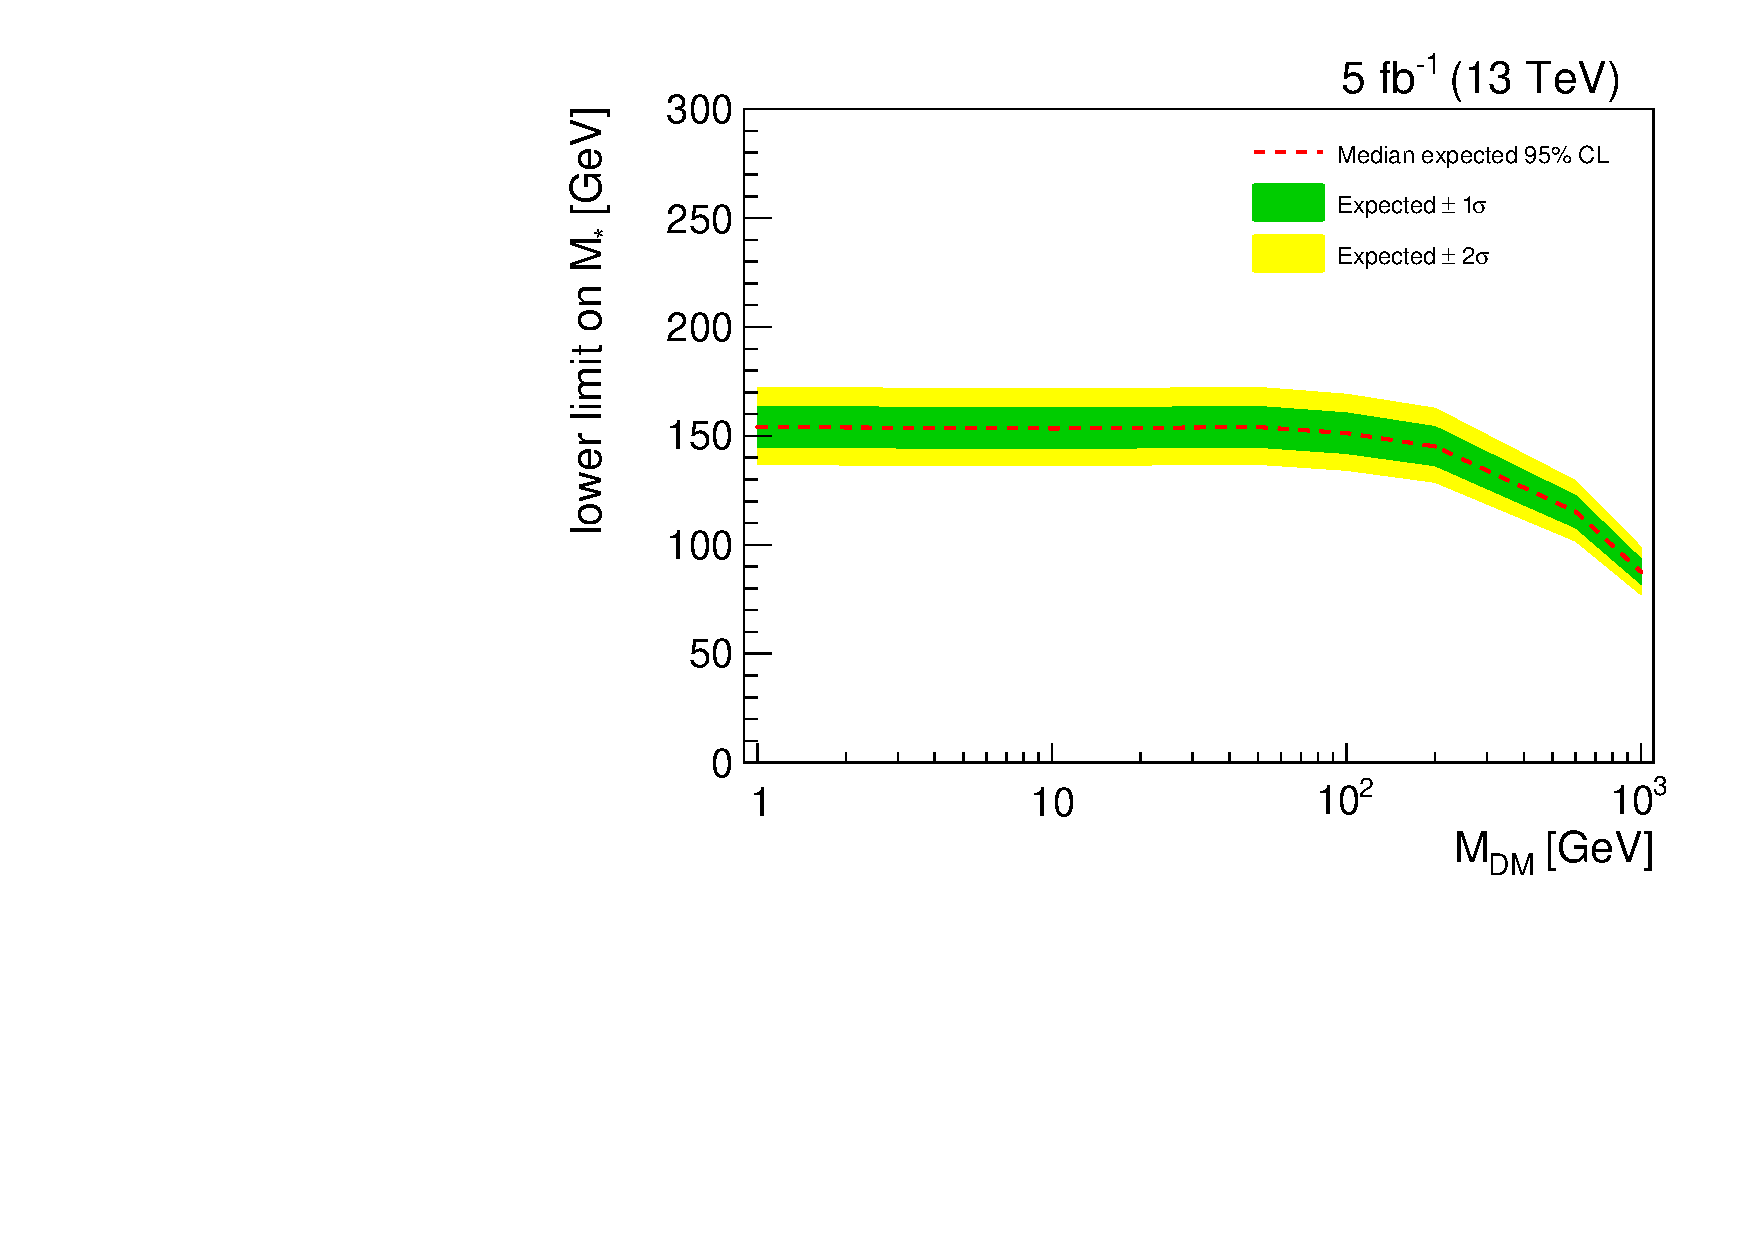
\includegraphics[width=0.32\textwidth]{figures/mstarLimit_hadronic_incl_shape.pdf}}
  \subfigure[Semileptonic]{\label{subfig:semilept_incl_shapem}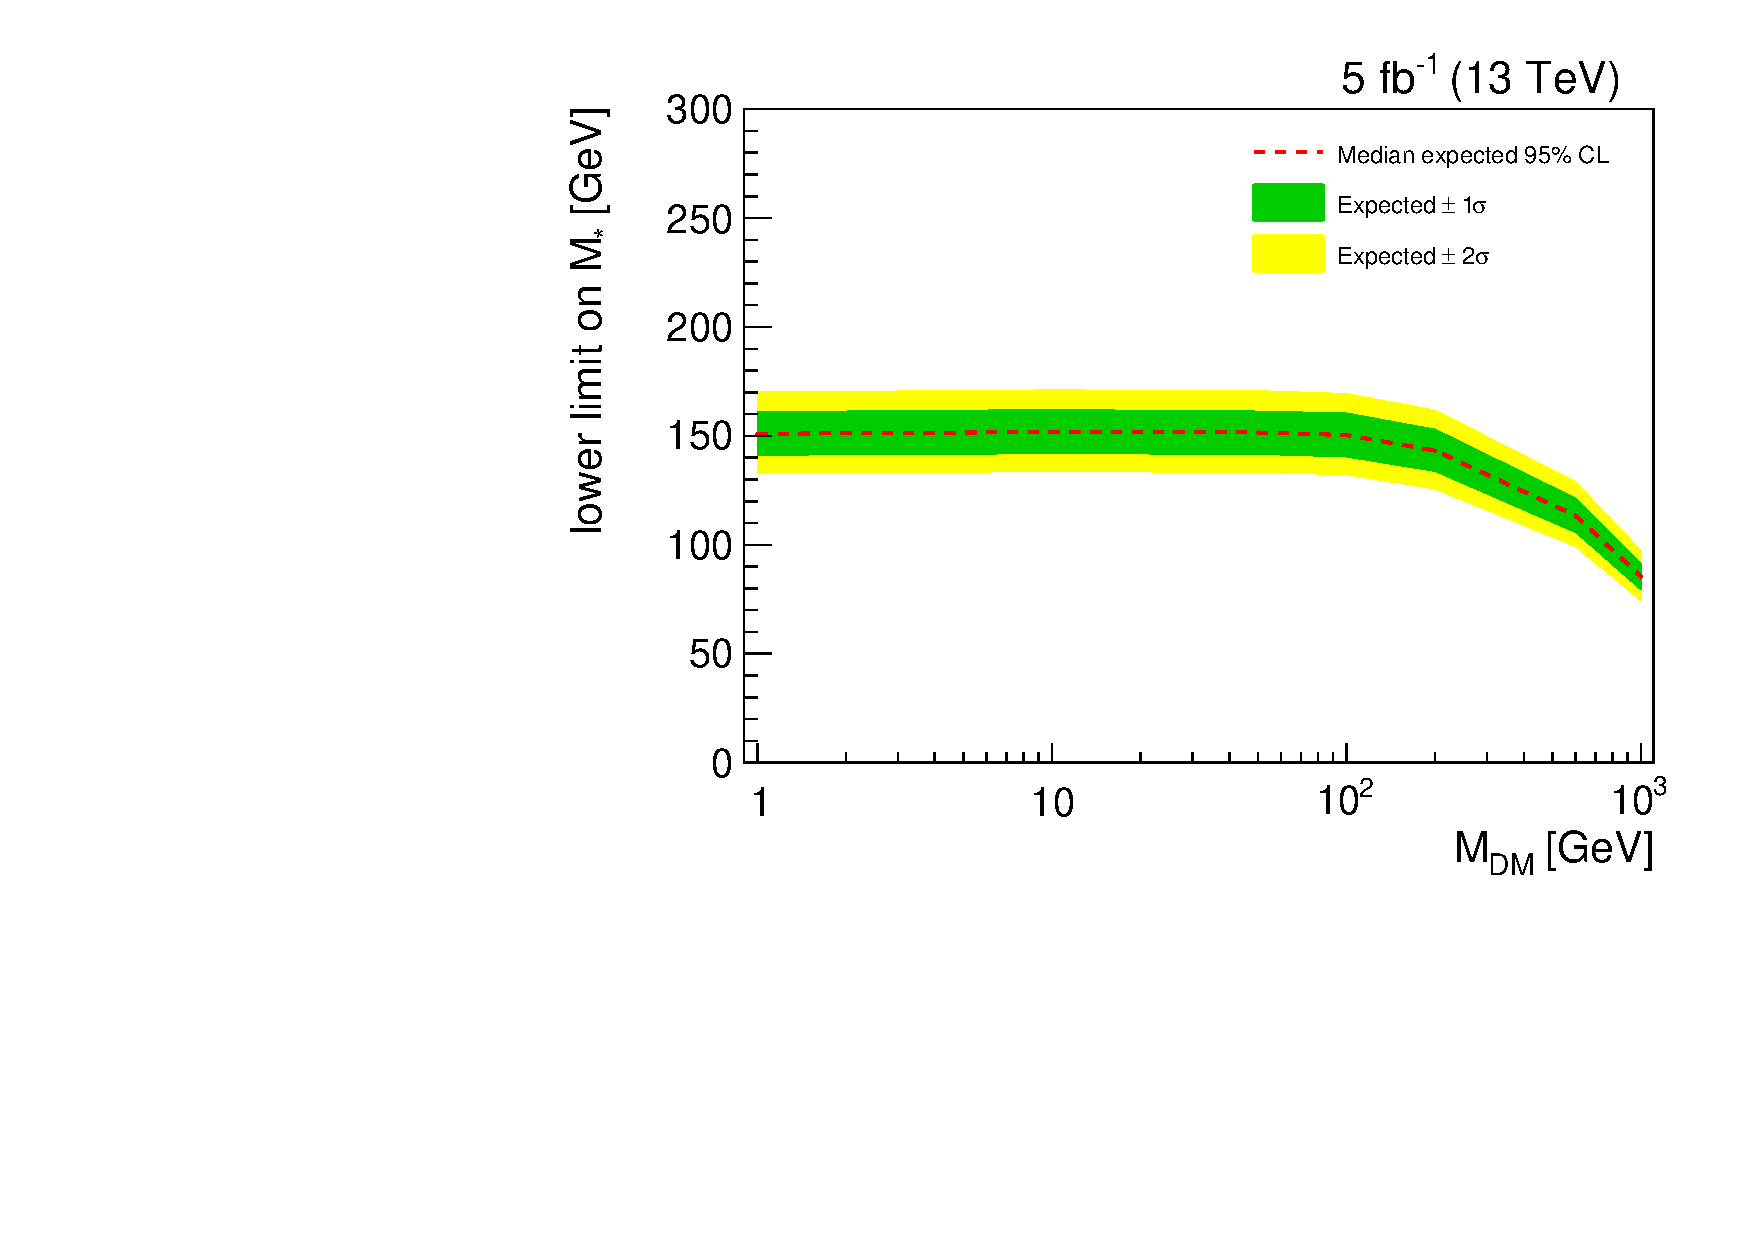
\includegraphics[width=0.32\textwidth]{figures/mstarLimit_semilept_incl_shape.pdf}}
  \subfigure[Combined]{\label{subfig:combined_incl_shapem}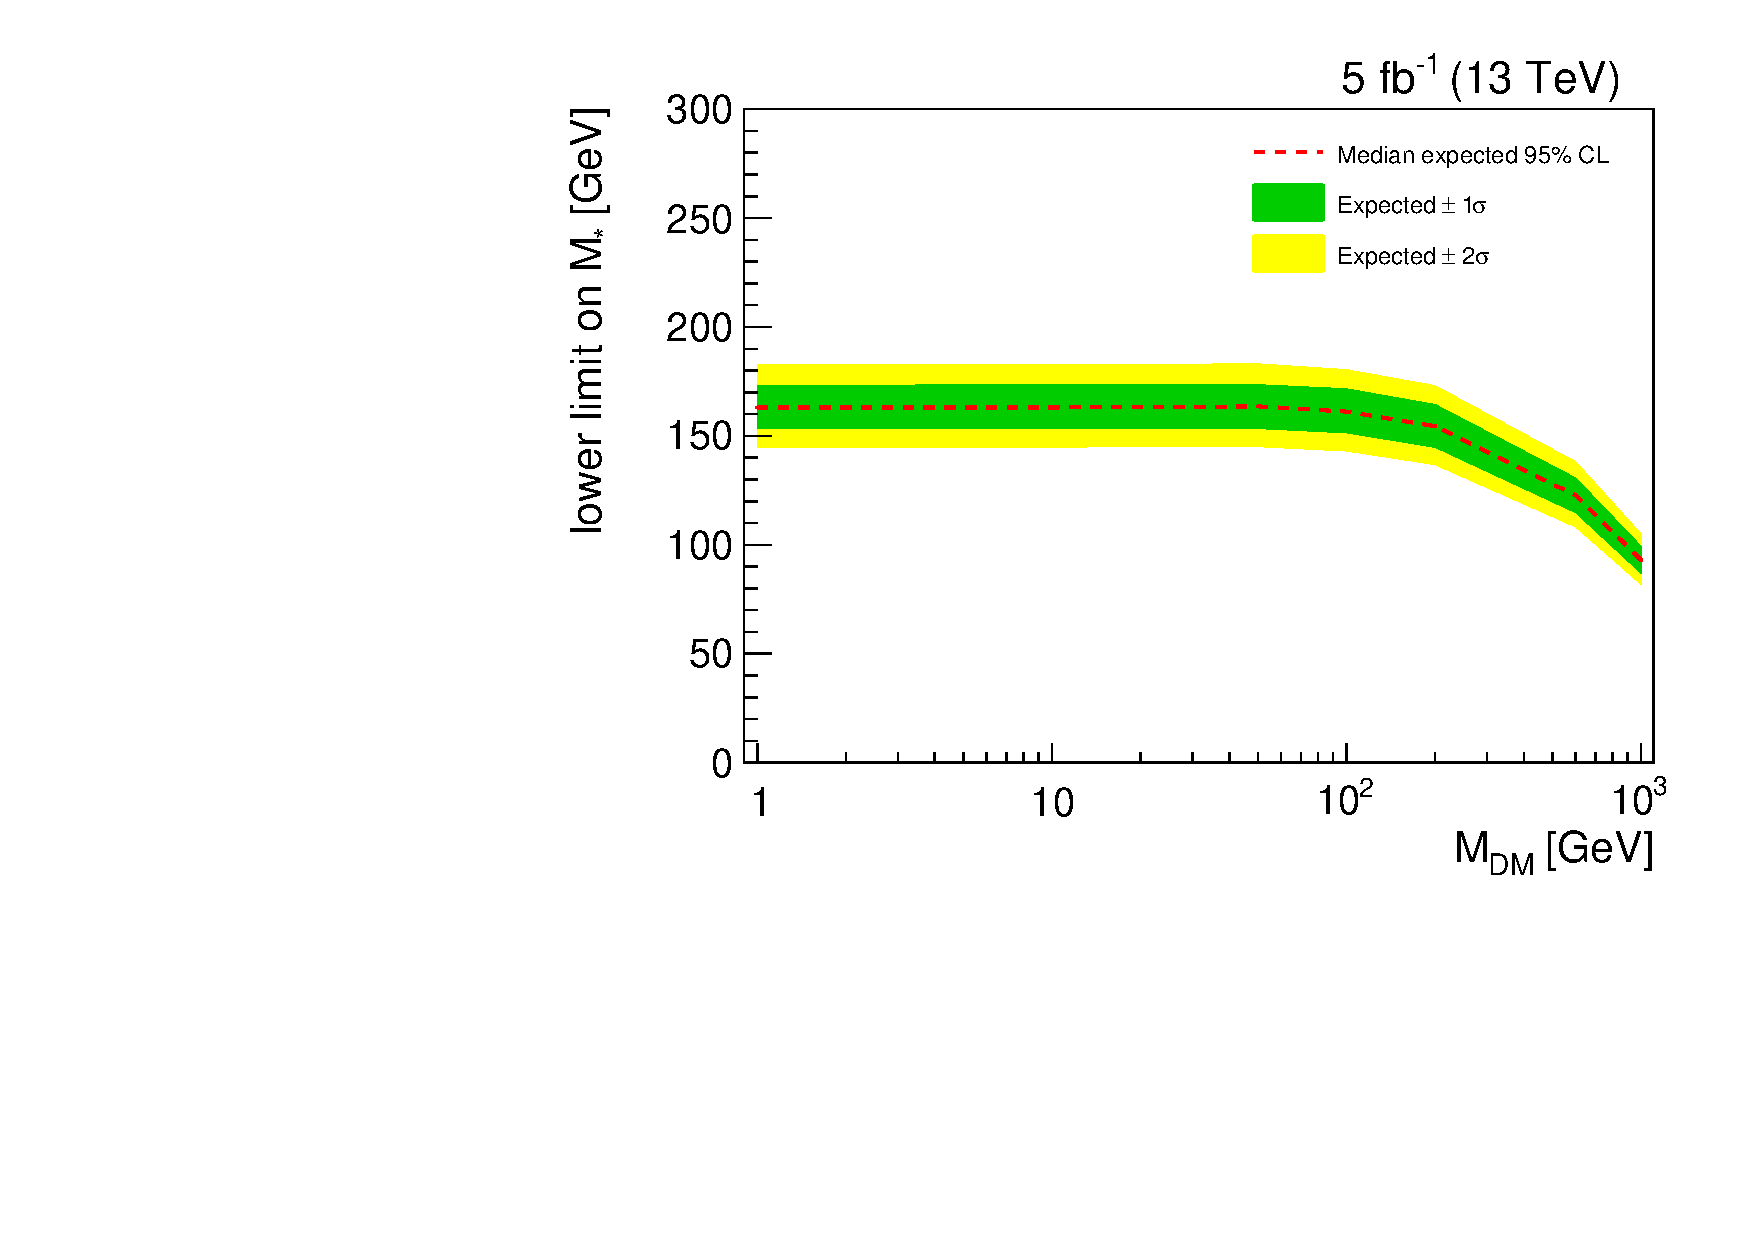
\includegraphics[width=0.32\textwidth]{figures/mstarLimit_incl_shape.pdf}}
  \caption{Expected lower limits on $M_*$ for the inclusive selections: \subref{subfig:hadronic_incl_shapem} hadronic channel, \subref{subfig:semilept_incl_shapem} semileptonic channel, and \subref{subfig:combined_incl_shapem} combination of both channels.}
  \label{fig:mstarlimits_incl_shape}
\end{center}
\end{figure}

The limits for the shape analysis is also performed on the top-tagging selections. The limits on the cross section ratio in each of the categories for the hadronic channel and for the semileptonic channel are shown in Fig.~\ref{fig:rlimits_hadronic_toptag_shape} and Fig.~\ref{fig:rlimits_semilept_toptag_shape}, respectively. For the hadronic channel, the most sensitive category is the Boosted-Resolved category.

\begin{figure}[htbp]
\begin{center}
  \subfigure[Boosted, Boosted]{\label{subfig:bst_bst}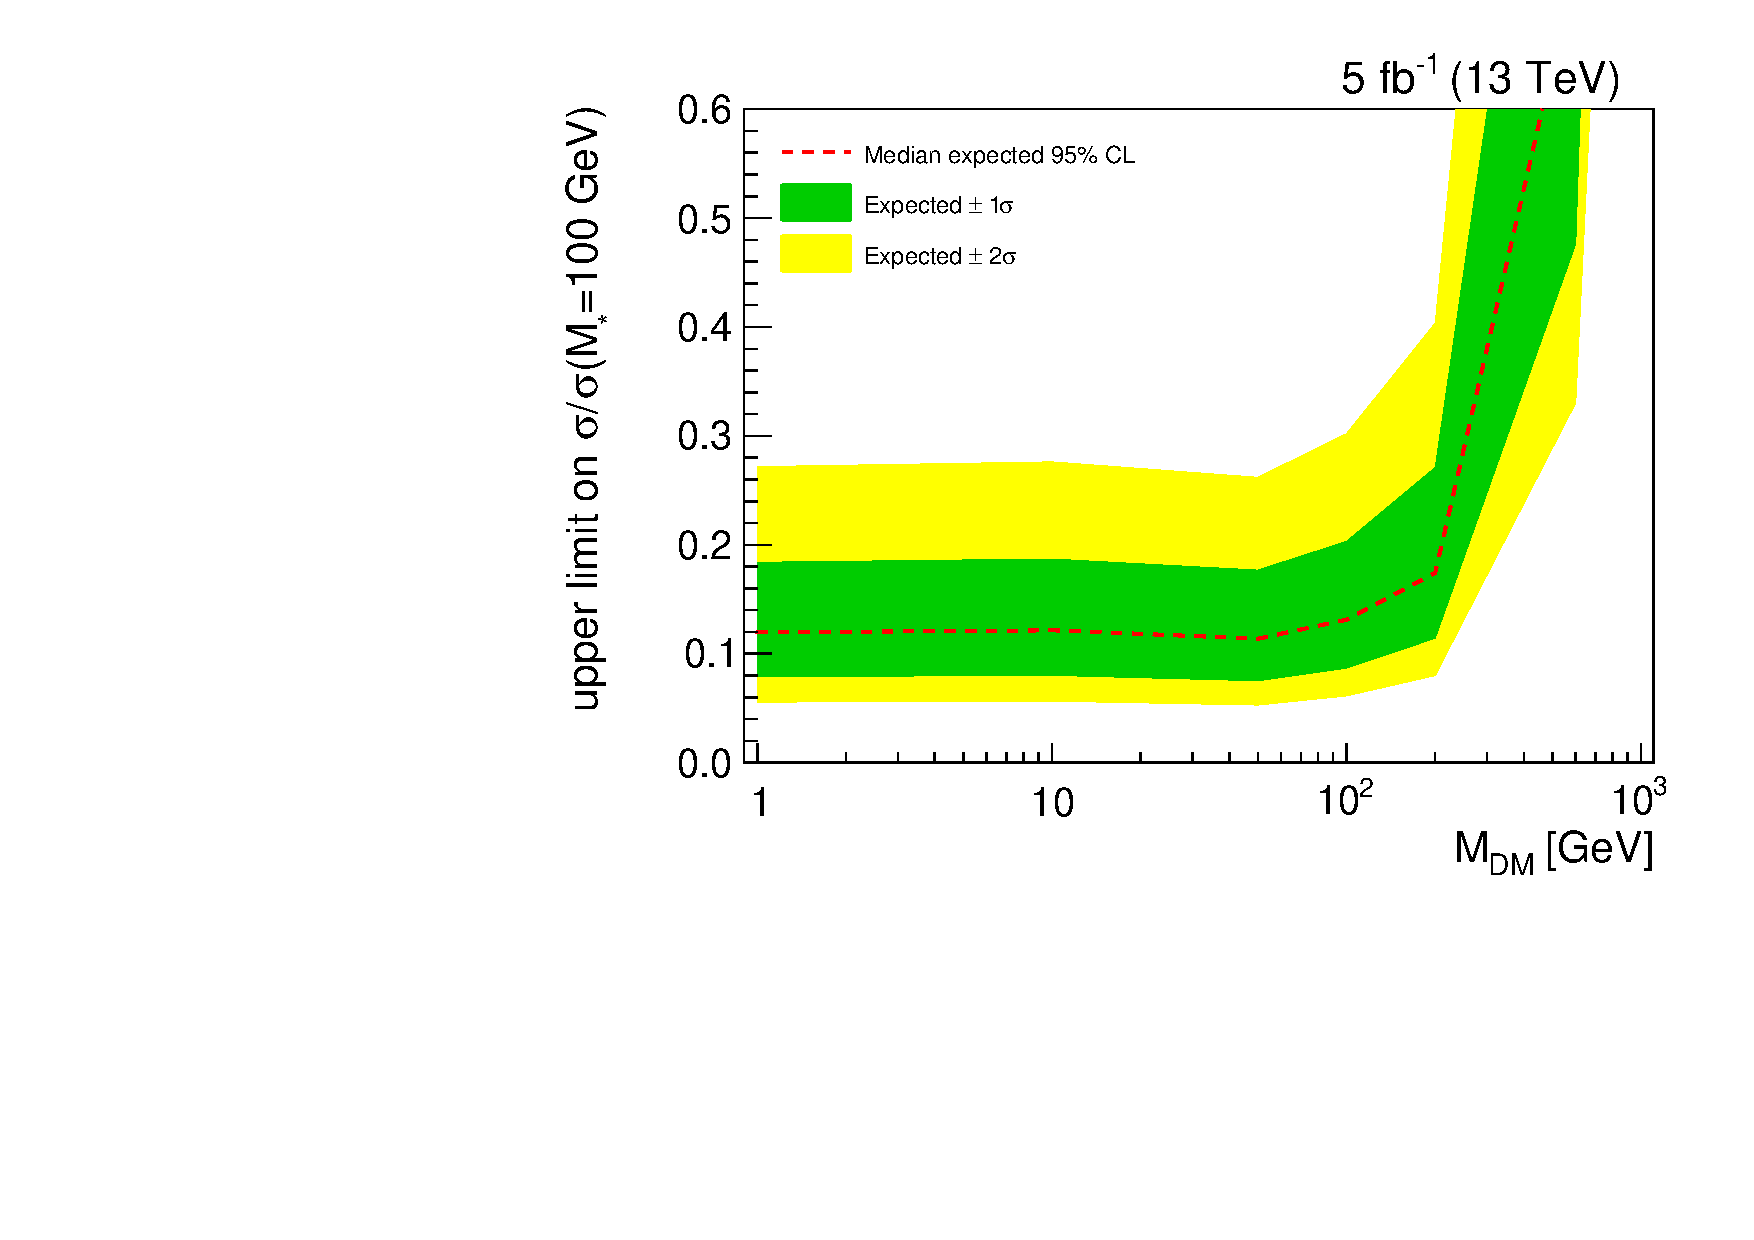
\includegraphics[width=0.32\textwidth]{figures/rLimit_hadronic_bst_bst_shape.pdf}}
  \subfigure[Boosted, Resolved]{\label{subfig:bst_res}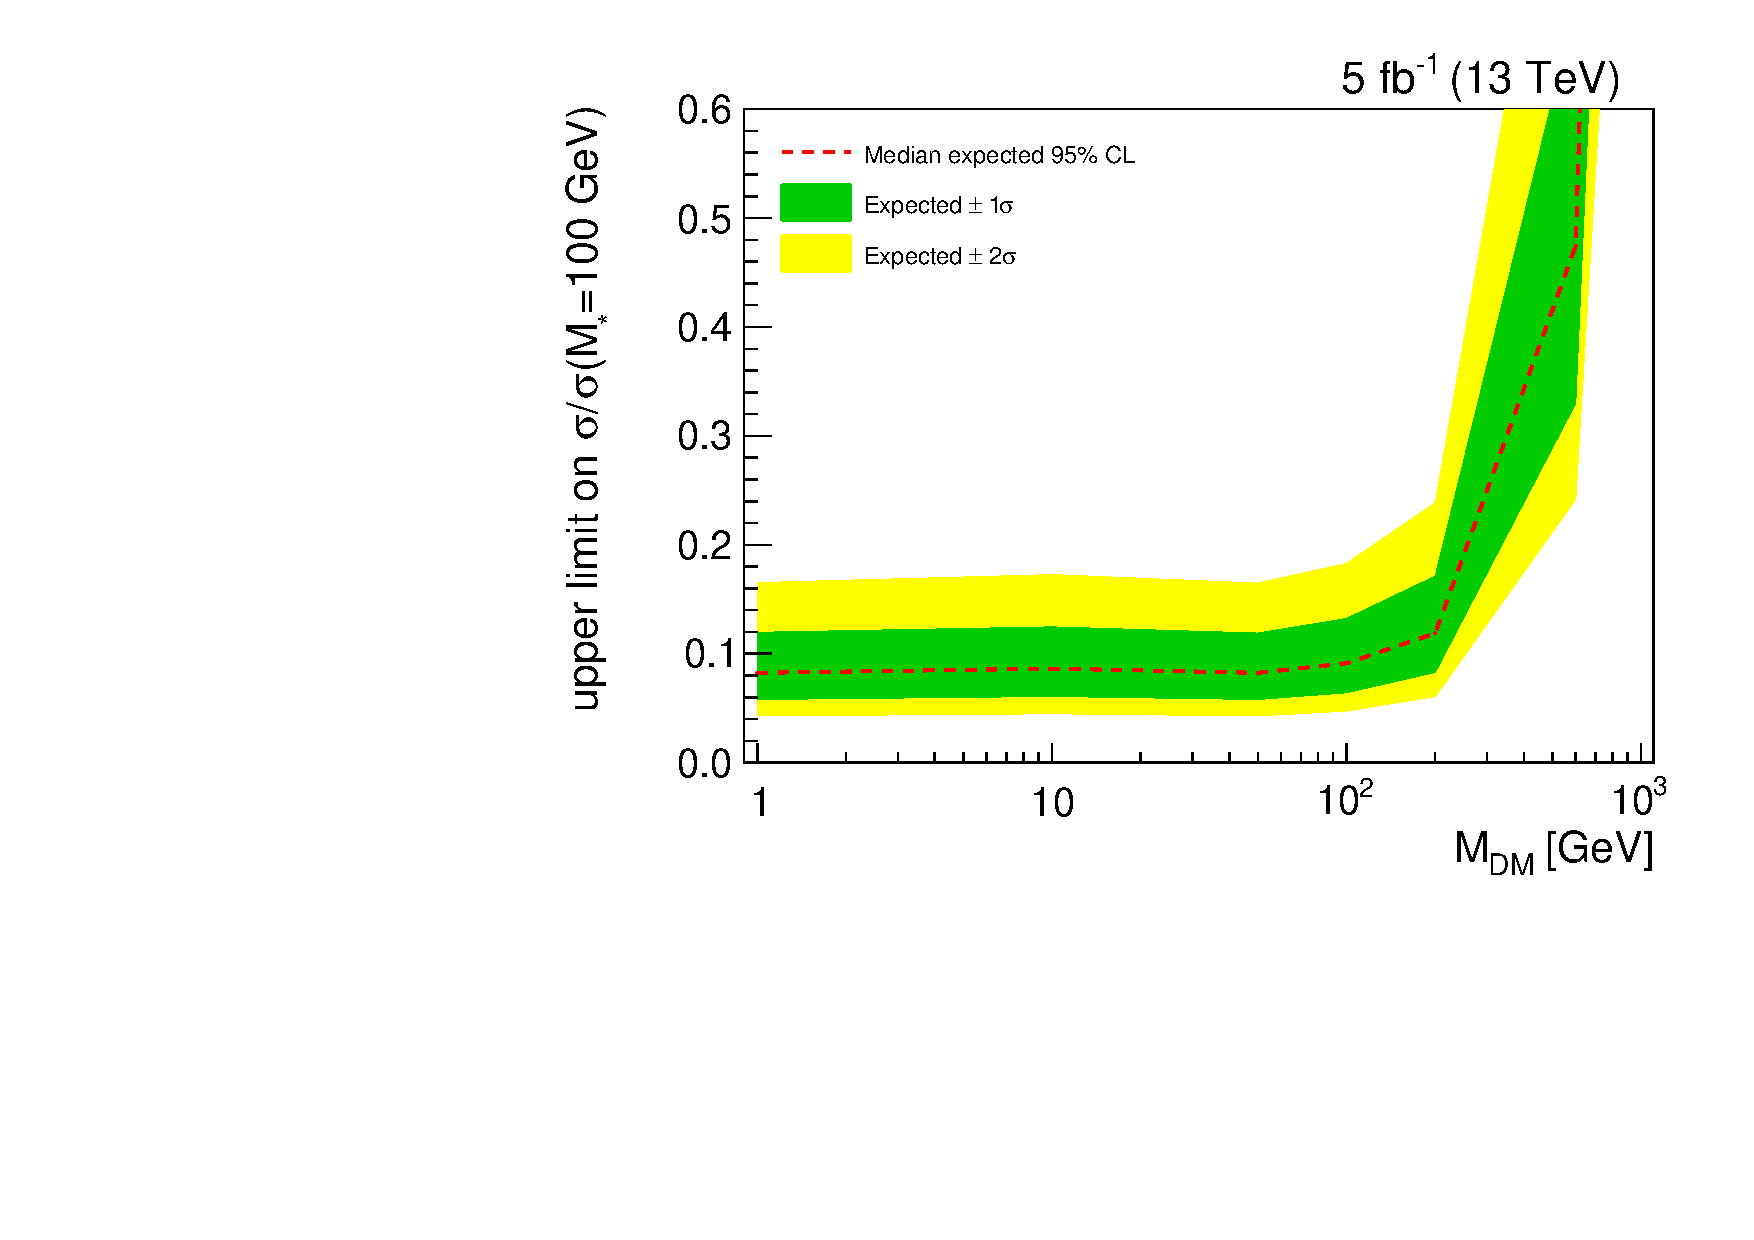
\includegraphics[width=0.32\textwidth]{figures/rLimit_hadronic_bst_res_shape.pdf}}
  \subfigure[Resolved, Resolved]{\label{subfig:res_res}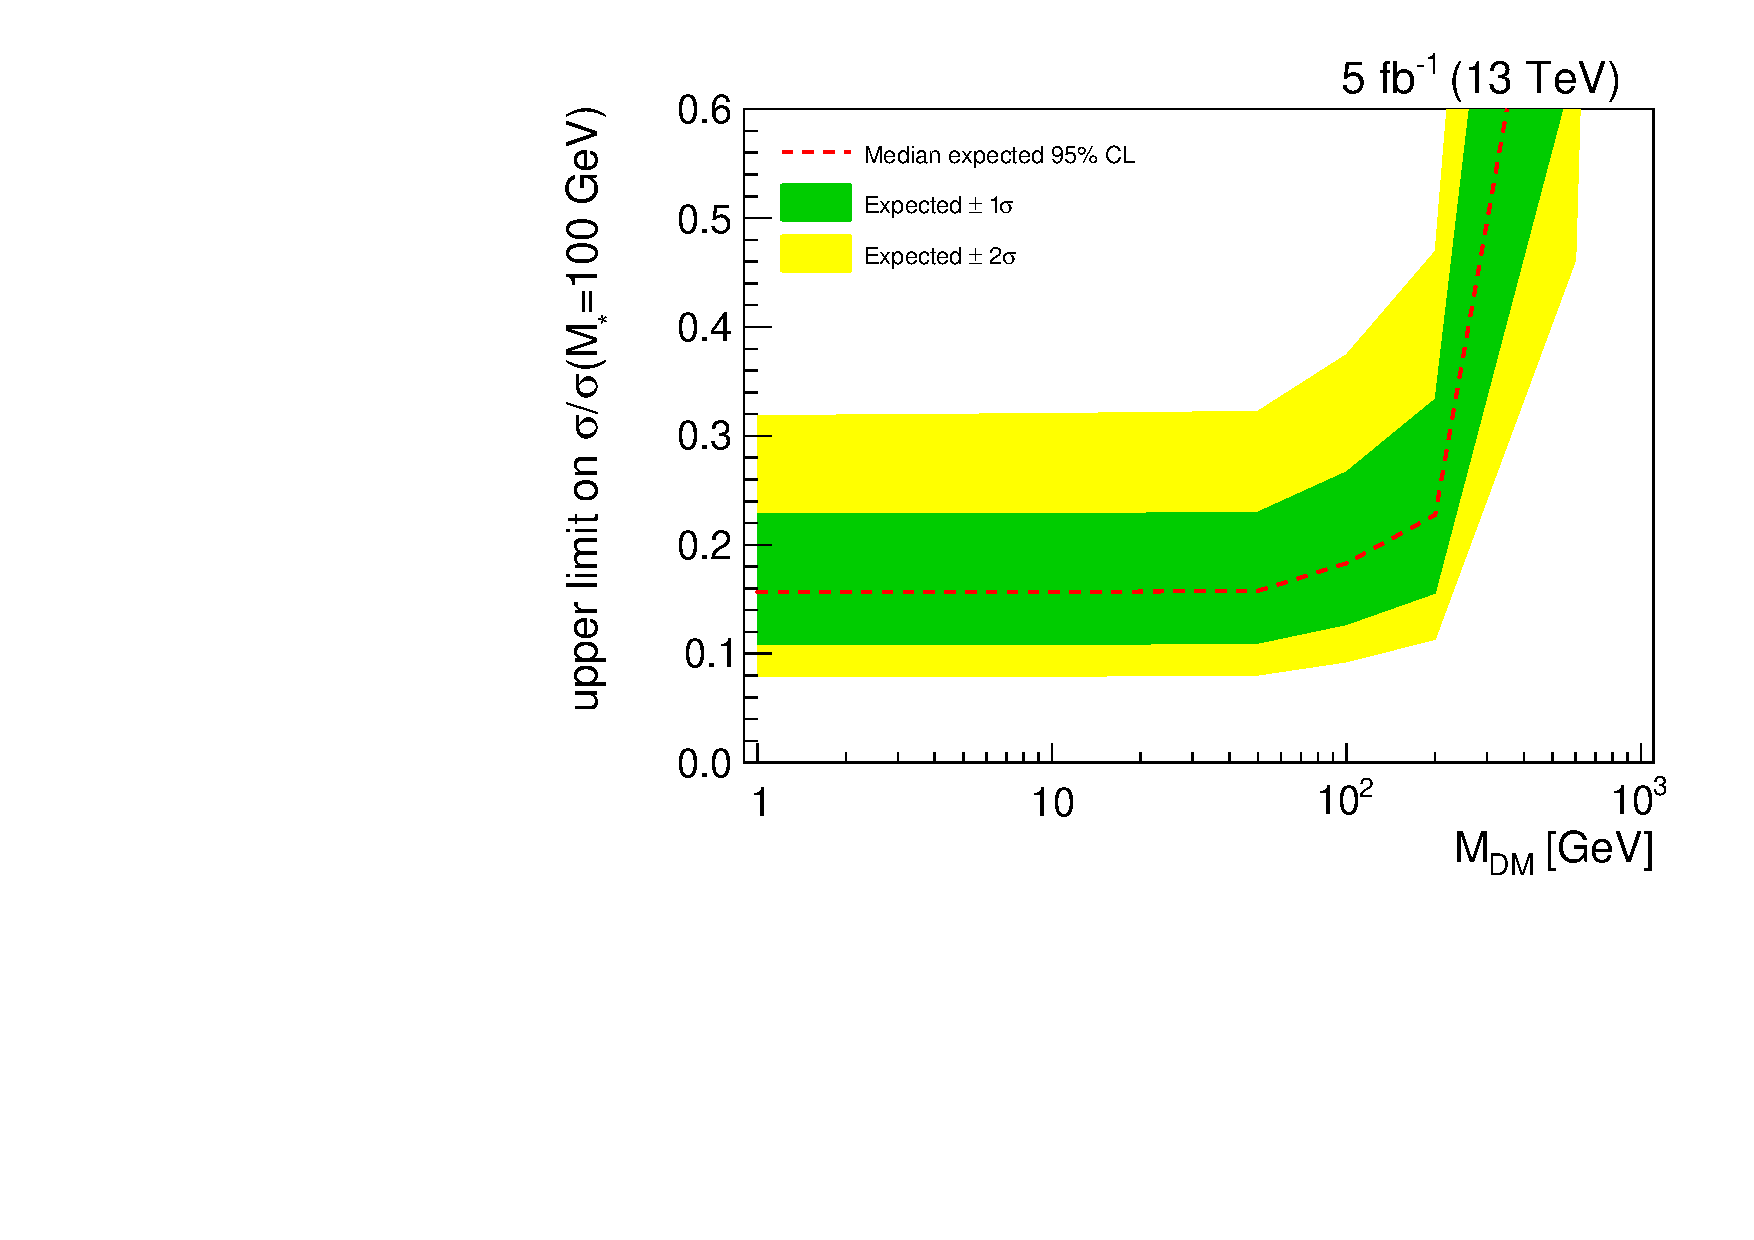
\includegraphics[width=0.32\textwidth]{figures/rLimit_hadronic_res_res_shape.pdf}}
  \caption{Expected upper limits on the cross section ratio relative to $M_*=100\:\GeV$ for each top tagging category in the hadronic channel: \subref{subfig:bst_bst} Boosted-Boosted, \subref{subfig:bst_res} Boosted-Resolved, and \subref{subfig:res_res} Resolved-Resolved.}
  \label{fig:rlimits_hadronic_toptag_shape}
\end{center}
\end{figure}

\begin{figure}[htbp]
\begin{center}
  \subfigure[Boosted]{\label{subfig:boosted}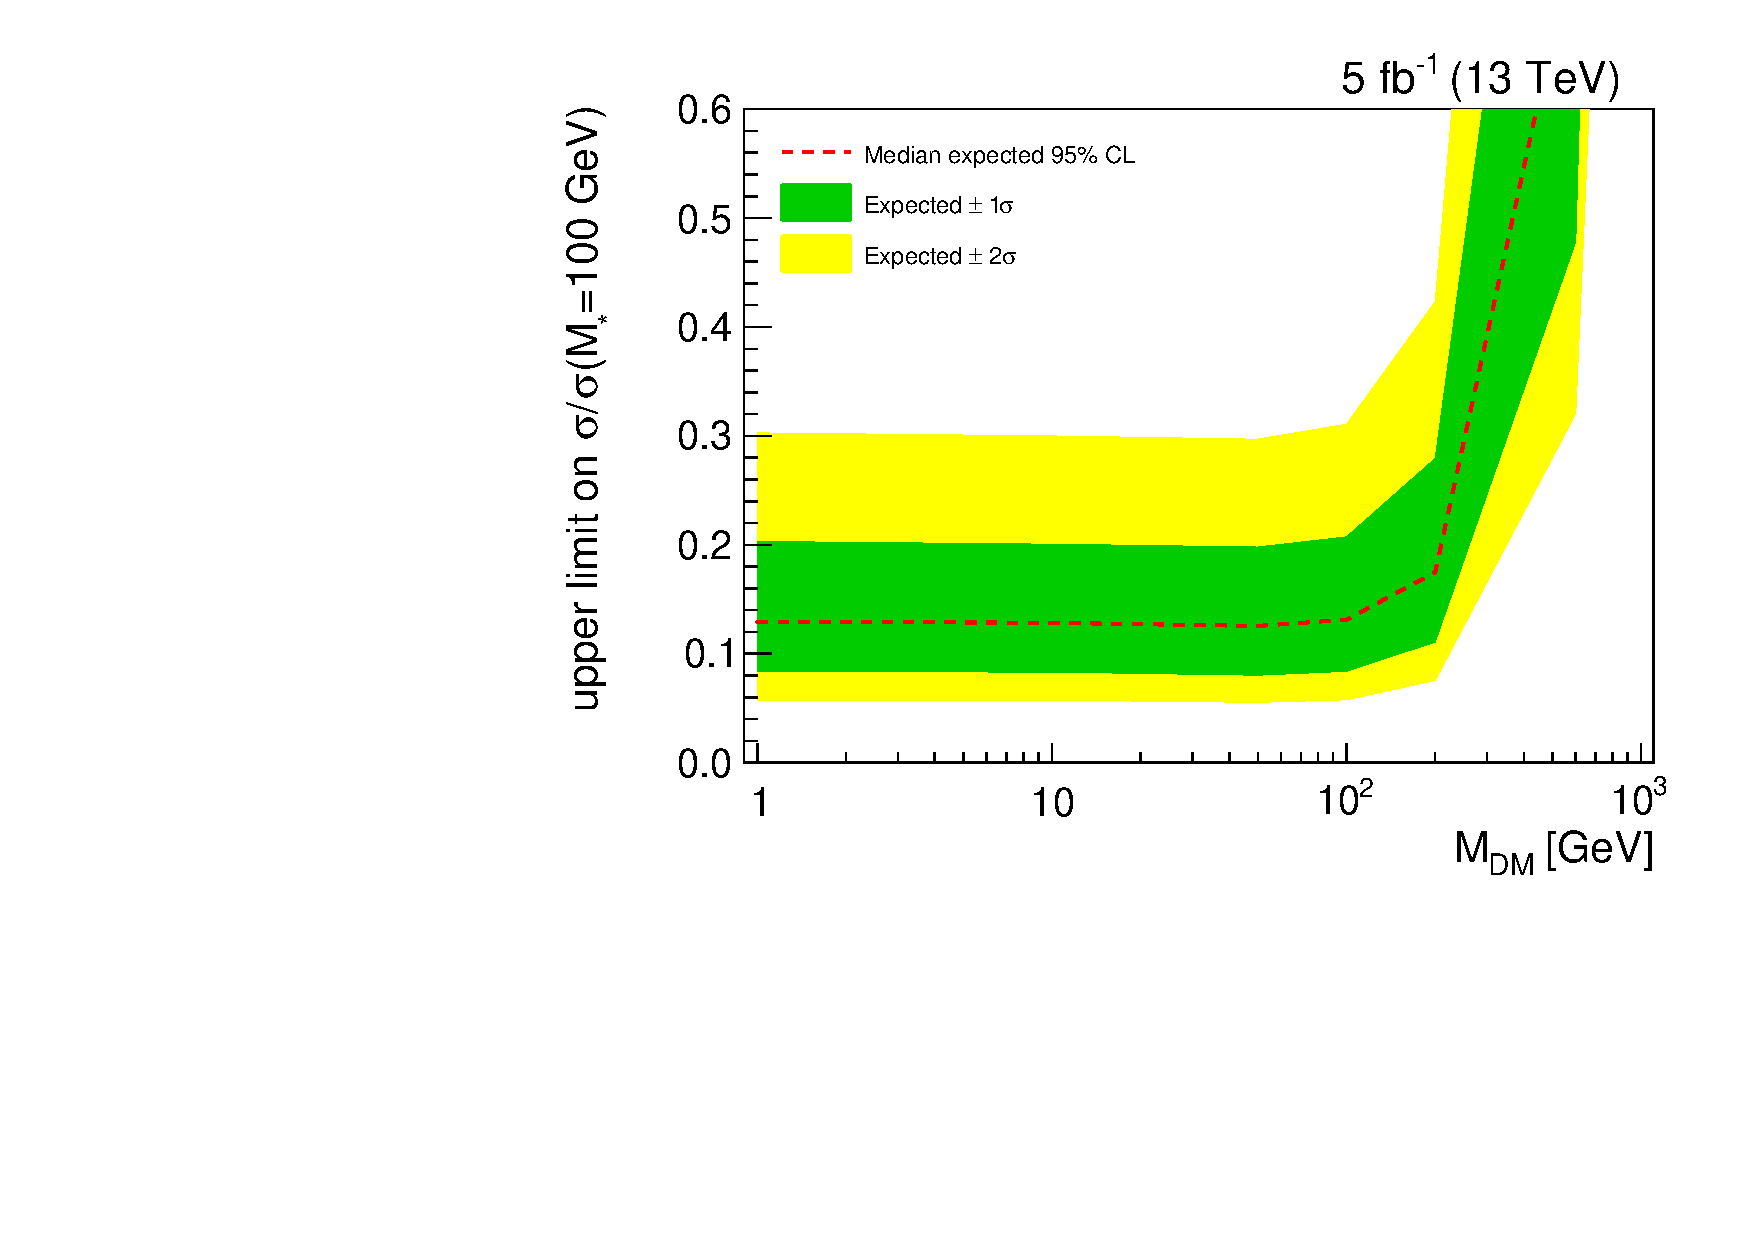
\includegraphics[width=0.32\textwidth]{figures/rLimit_semilept_boosted_shape.pdf}}
  \subfigure[Resolved]{\label{subfig:resolved}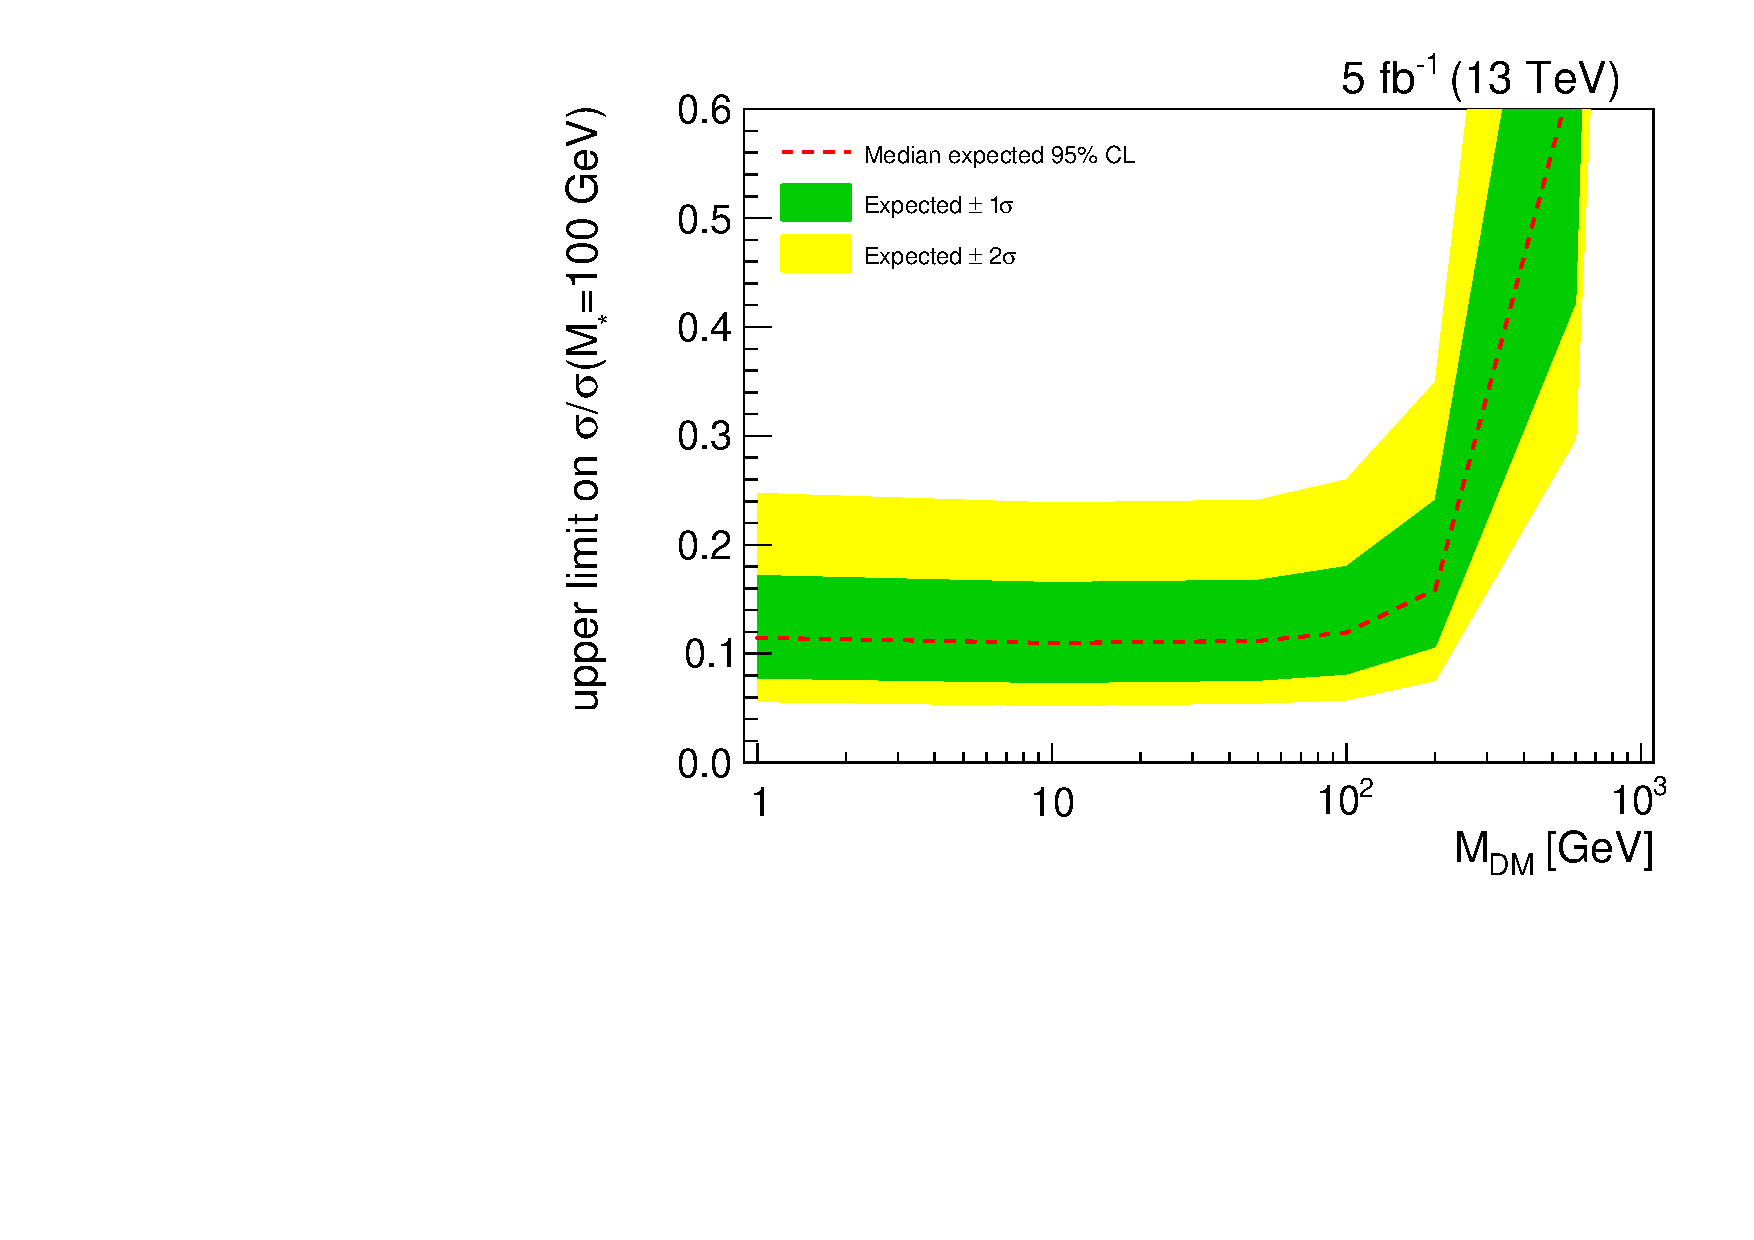
\includegraphics[width=0.32\textwidth]{figures/rLimit_semilept_resolved_shape.pdf}}
  \caption{Expected upper limits on the cross section ratio relative to $M_*=100\:\GeV$ for each top tagging category in the semileptonic channel: \subref{subfig:boosted} Boosted, and \subref{subfig:resolved} Resolved.}
  \label{fig:rlimits_semilept_toptag_shape}
\end{center}
\end{figure}

The limits on the cross section ratio and $M_*$ from combining the top-tagged categories are shown in Fig.~\ref{fig:rlimits_combo_shape} and Fig.~\ref{fig:mstarlimits_combo_shape}, respectively. The top-tagging categories bring an improvement to the sensitivity of about $20\%$ for the hadronic channel and about $10\%$ for the semileptonic channel.

\begin{figure}[htbp]
\begin{center}
  \subfigure[Hadronic]{\label{subfig:hadronic_cat_shape}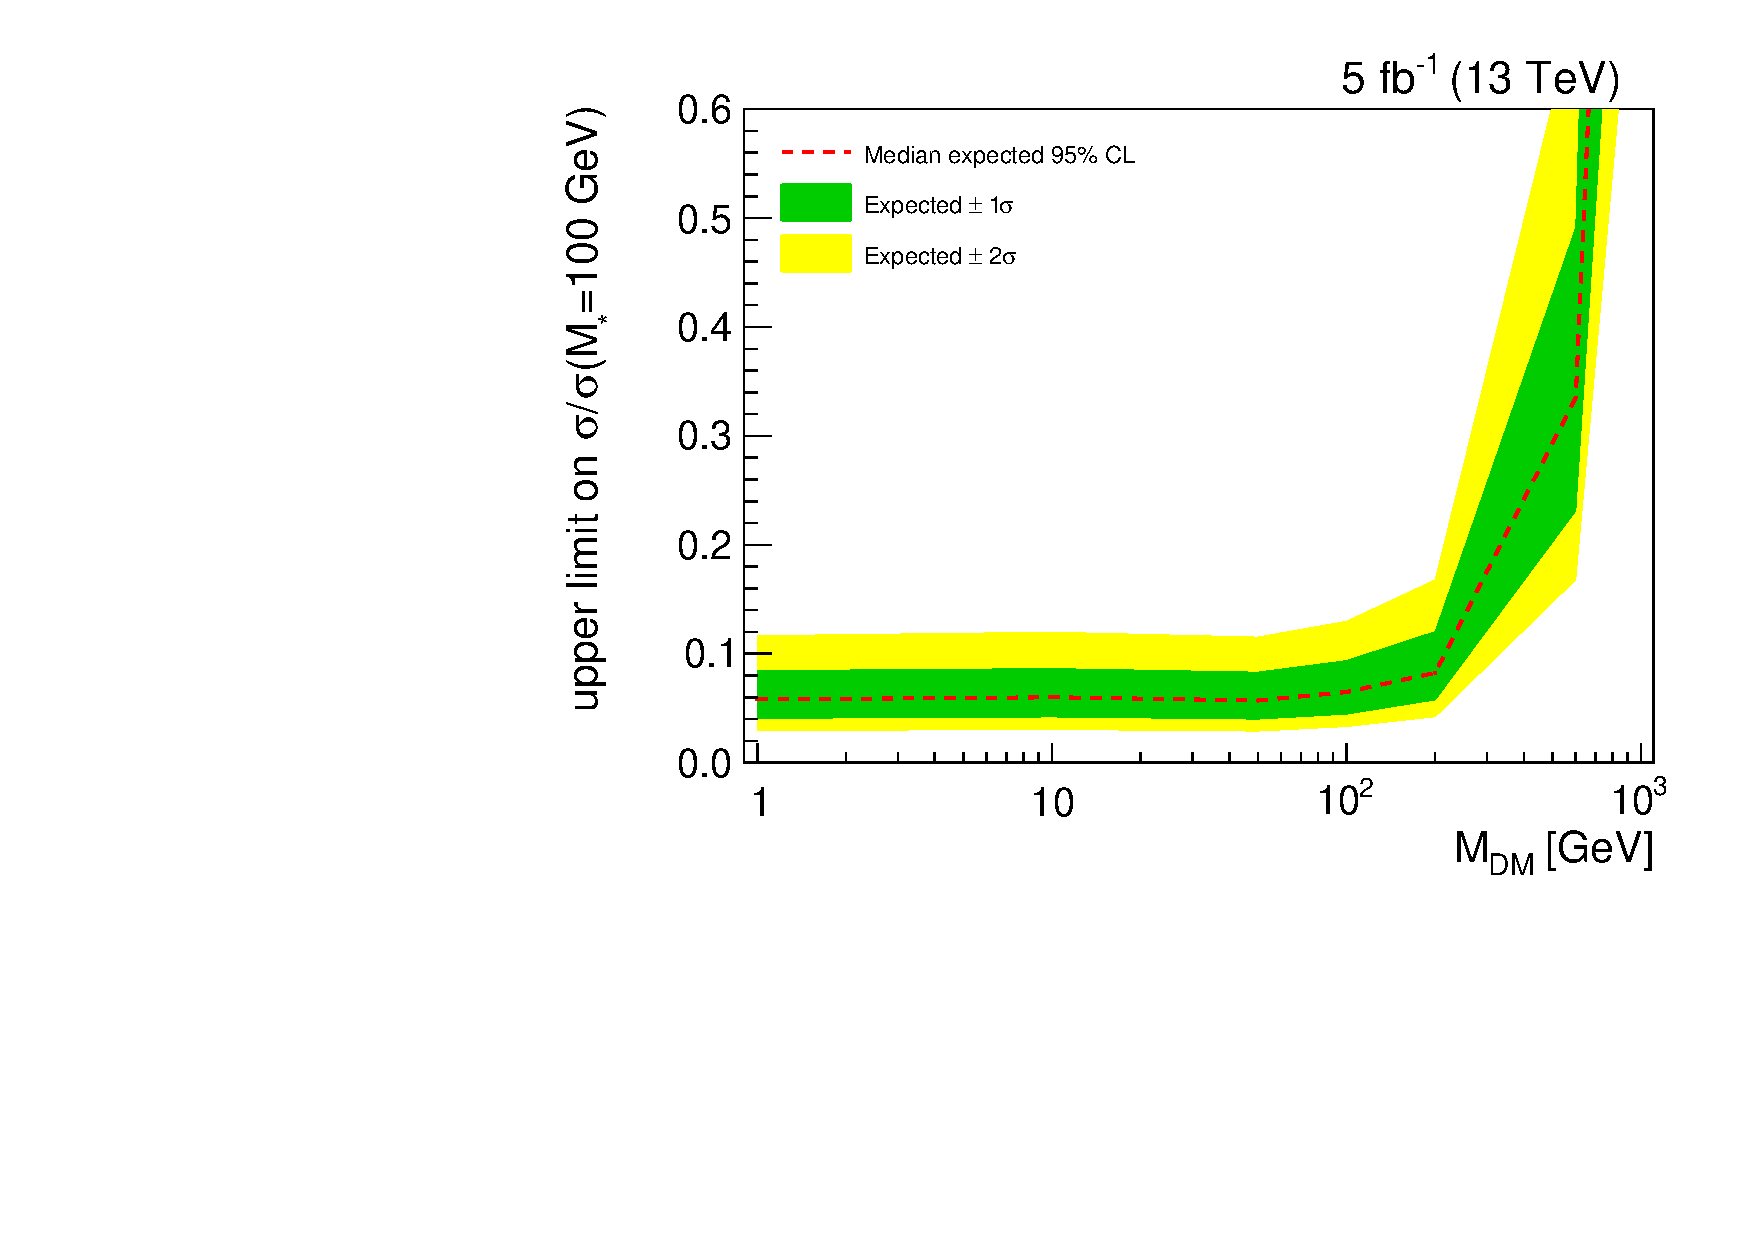
\includegraphics[width=0.32\textwidth]{figures/rLimit_hadronic_combo_shape.pdf}}
  \subfigure[Semileptonic]{\label{subfig:semilept_cat_shape}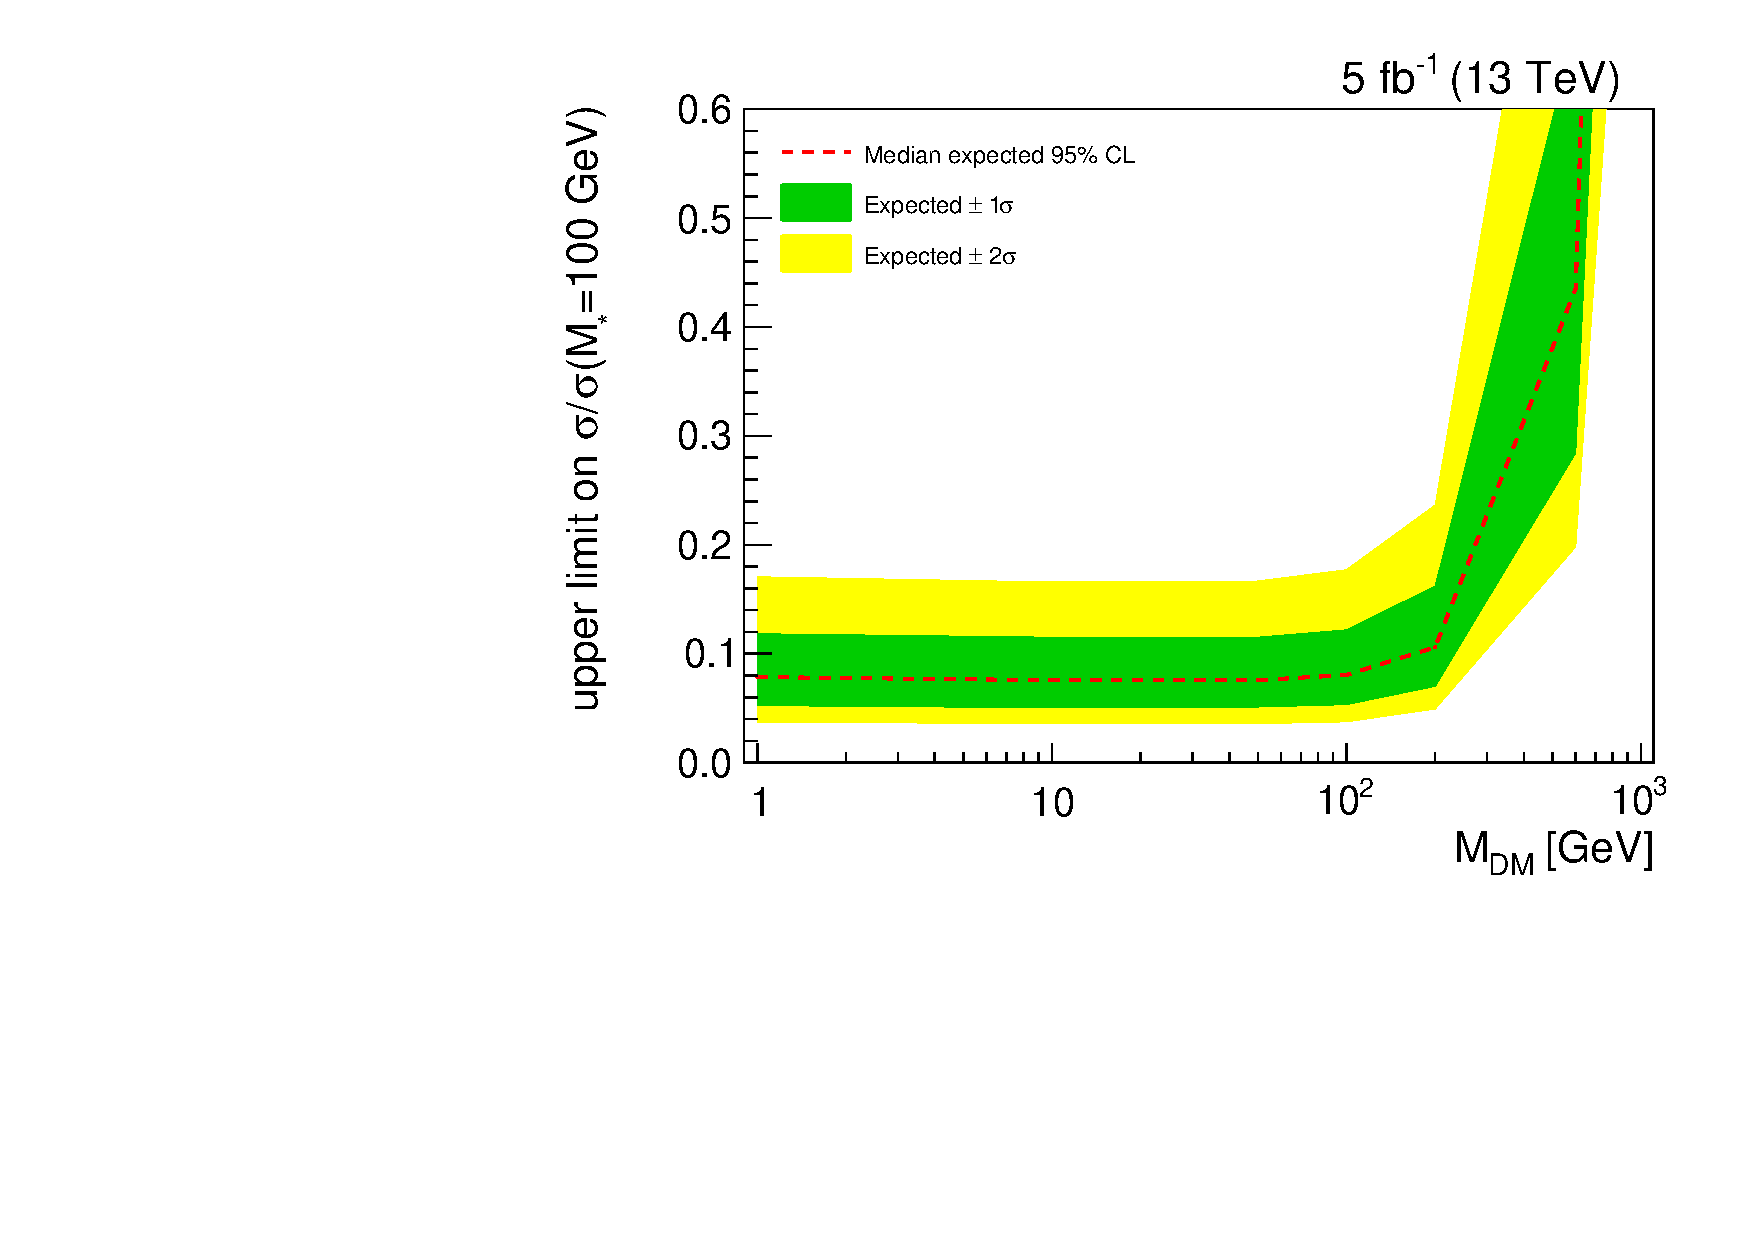
\includegraphics[width=0.32\textwidth]{figures/rLimit_semilept_combo_shape.pdf}}
  \subfigure[Combined]{\label{subfig:combined_cat_shape}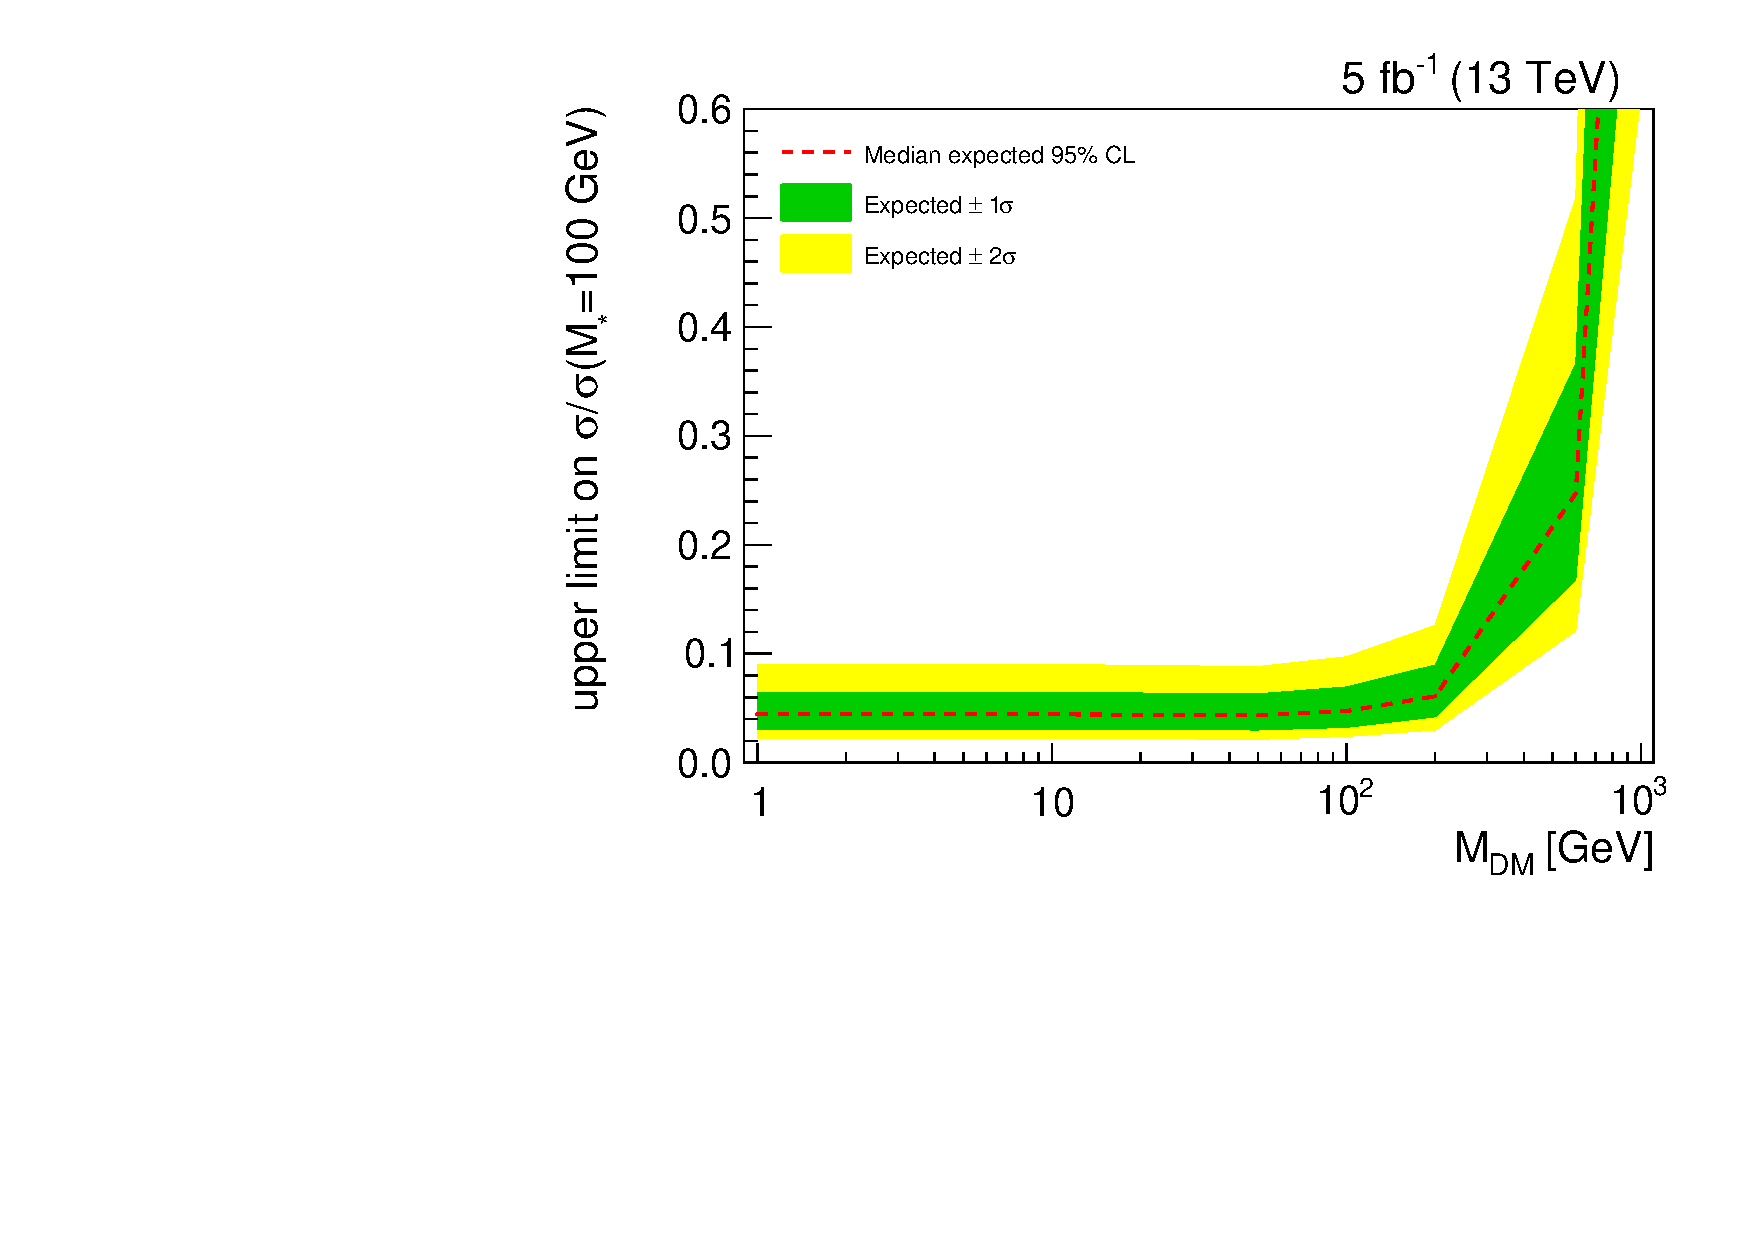
\includegraphics[width=0.32\textwidth]{figures/rLimit_combo_shape.pdf}}
  \caption{Expected upper limits on the cross section ratio relative to $M_*=100\:\GeV$ from combining all top tagging categories: \subref{subfig:hadronic_cat_shape} hadronic channel, \subref{subfig:semilept_cat_shape} semileptonic channel, and \subref{subfig:combined_cat_shape} combination of both channels.}
  \label{fig:rlimits_combo_shape}
\end{center}
\end{figure}

\begin{table}[!ht]
\centering
\begin{tabular}{|r|c|c|c|}
\hline
  $M_\chi$ $(\GeV)$ & Median & $\left[-1\sigma\, +1\sigma\right]$ & $\left[-2\sigma\, +2\sigma\right]$ \\
\hline
  $1$               & $0.0581$ & $\left[0.0407\, 0.0845\right]$ & $\left[0.0295\, 0.1166\right]$ \\
  $10$              & $0.0601$ & $\left[0.0420\, 0.0864\right]$ & $\left[0.0305\, 0.1198\right]$ \\
  $50$              & $0.0571$ & $\left[0.0400\, 0.0831\right]$ & $\left[0.0290\, 0.1153\right]$ \\
  $100$             & $0.0649$ & $\left[0.0446\, 0.0937\right]$ & $\left[0.0332\, 0.1298\right]$ \\
  $200$             & $0.0825$ & $\left[0.0577\, 0.1203\right]$ & $\left[0.0422\, 0.1678\right]$ \\
  $600$             & $0.3350$ & $\left[0.2313\, 0.4912\right]$ & $\left[0.1681\, 0.6910\right]$ \\
  $1000$            & $1.6797$ & $\left[1.1520\, 2.5032\right]$ & $\left[0.8300\, 3.5511\right]$ \\
\hline
\end{tabular}
\caption{Expected upper limits on the cross section ratio relative to $M_*=100\:\GeV$ for inclusive selection in the hadronic channel.}
\label{tab:rLimits_hadronic_comboshape}
\end{table}

\begin{table}[!ht]
\centering
\begin{tabular}{|r|c|c|c|}
\hline
  $M_\chi$ $(\GeV)$ & Median & $\left[-1\sigma\, +1\sigma\right]$ & $\left[-2\sigma\, +2\sigma\right]$ \\
\hline
  $1$               & $0.0786$ & $\left[0.0524\, 0.1184\right]$ & $\left[0.0372\, 0.1707\right]$ \\
  $10$              & $0.0757$ & $\left[0.0504\, 0.1152\right]$ & $\left[0.0358\, 0.1659\right]$ \\
  $50$              & $0.0757$ & $\left[0.0511\, 0.1152\right]$ & $\left[0.0358\, 0.1668\right]$ \\
  $100$             & $0.0806$ & $\left[0.0533\, 0.1220\right]$ & $\left[0.0375\, 0.1772\right]$ \\
  $200$             & $0.1060$ & $\left[0.0701\, 0.1621\right]$ & $\left[0.0493\, 0.2365\right]$ \\
  $600$             & $0.4355$ & $\left[0.2844\, 0.6769\right]$ & $\left[0.1982\, 0.9981\right]$ \\
  $1000$            & $2.3828$ & $\left[1.5442\, 3.7410\right]$ & $\left[1.0658\, 5.5755\right]$ \\
\hline
\end{tabular}
\caption{Expected upper limits on the cross section ratio relative to $M_*=100\:\GeV$ for inclusive selection in the semileptonic channel.}
\label{tab:rLimits_semilept_comboshape}
\end{table}

\begin{table}[!ht]
\centering
\begin{tabular}{|r|c|c|c|}
\hline
  $M_\chi$ $(\GeV)$ & Median & $\left[-1\sigma\, +1\sigma\right]$ & $\left[-2\sigma\, +2\sigma\right]$ \\
\hline
  $1$               & $0.0444$ & $\left[0.0304\, 0.0646\right]$ & $\left[0.0226\, 0.0897\right]$ \\
  $10$              & $0.0444$ & $\left[0.0304\, 0.0646\right]$ & $\left[0.0226\, 0.0902\right]$ \\
  $50$              & $0.0435$ & $\left[0.0300\, 0.0632\right]$ & $\left[0.0214\, 0.0882\right]$ \\
  $100$             & $0.0474$ & $\left[0.0324\, 0.0696\right]$ & $\left[0.0241\, 0.0972\right]$ \\
  $200$             & $0.0610$ & $\left[0.0421\, 0.0897\right]$ & $\left[0.0300\, 0.1261\right]$ \\
  $600$             & $0.2471$ & $\left[0.1679\, 0.3662\right]$ & $\left[0.1211\, 0.5182\right]$ \\
  $1000$            & $1.2695$ & $\left[0.8563\, 1.8920\right]$ & $\left[0.6124\, 2.7147\right]$ \\
\hline
\end{tabular}
\caption{Expected upper limits on the cross section ratio relative to $M_*=100\:\GeV$ for combined hadronic and semileptonic channel.}
\label{tab:rLimits_comboshape}
\end{table}

\begin{figure}[htbp]
\begin{center}
  \subfigure[Hadronic]{\label{subfig:hadronic_cat_shapem}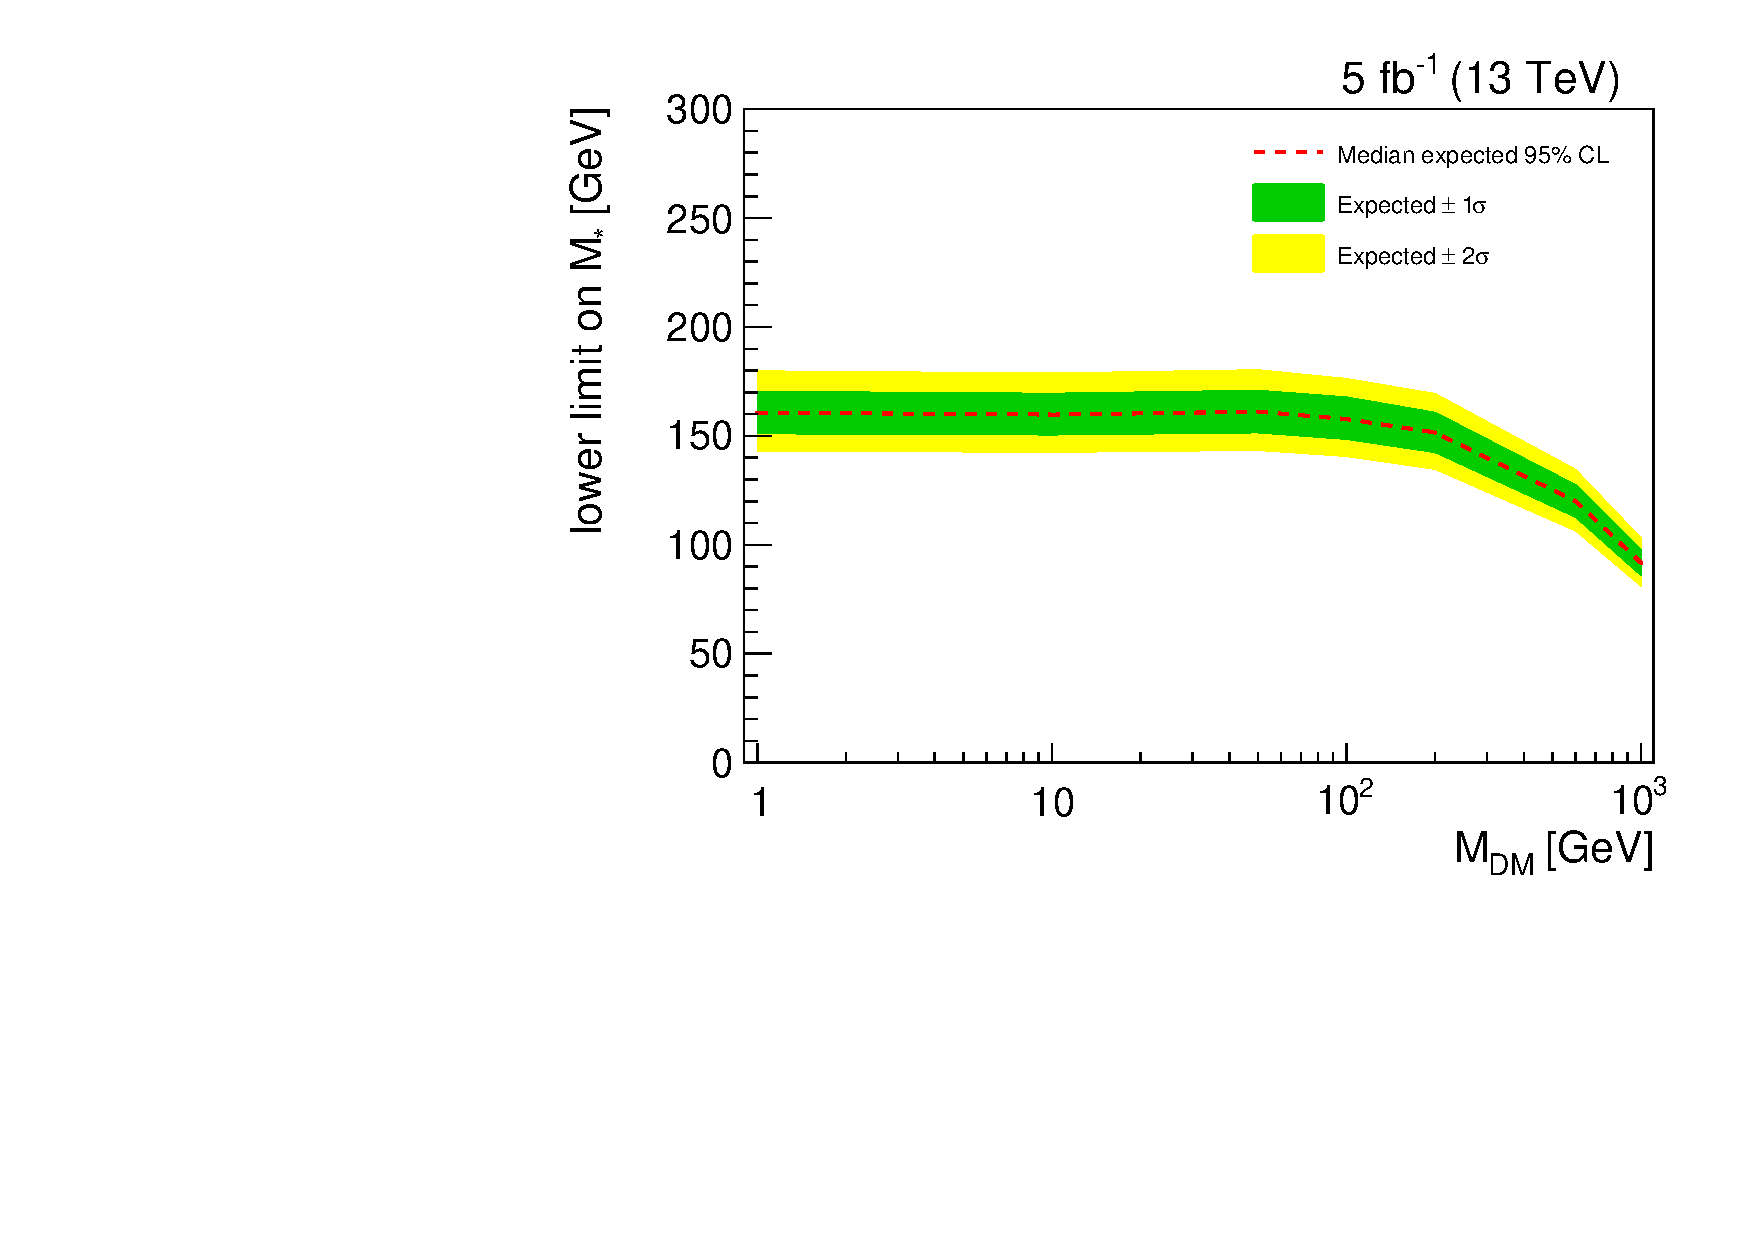
\includegraphics[width=0.32\textwidth]{figures/mstarLimit_hadronic_combo_shape.pdf}}
  \subfigure[Semileptonic]{\label{subfig:semilept_cat_shapem}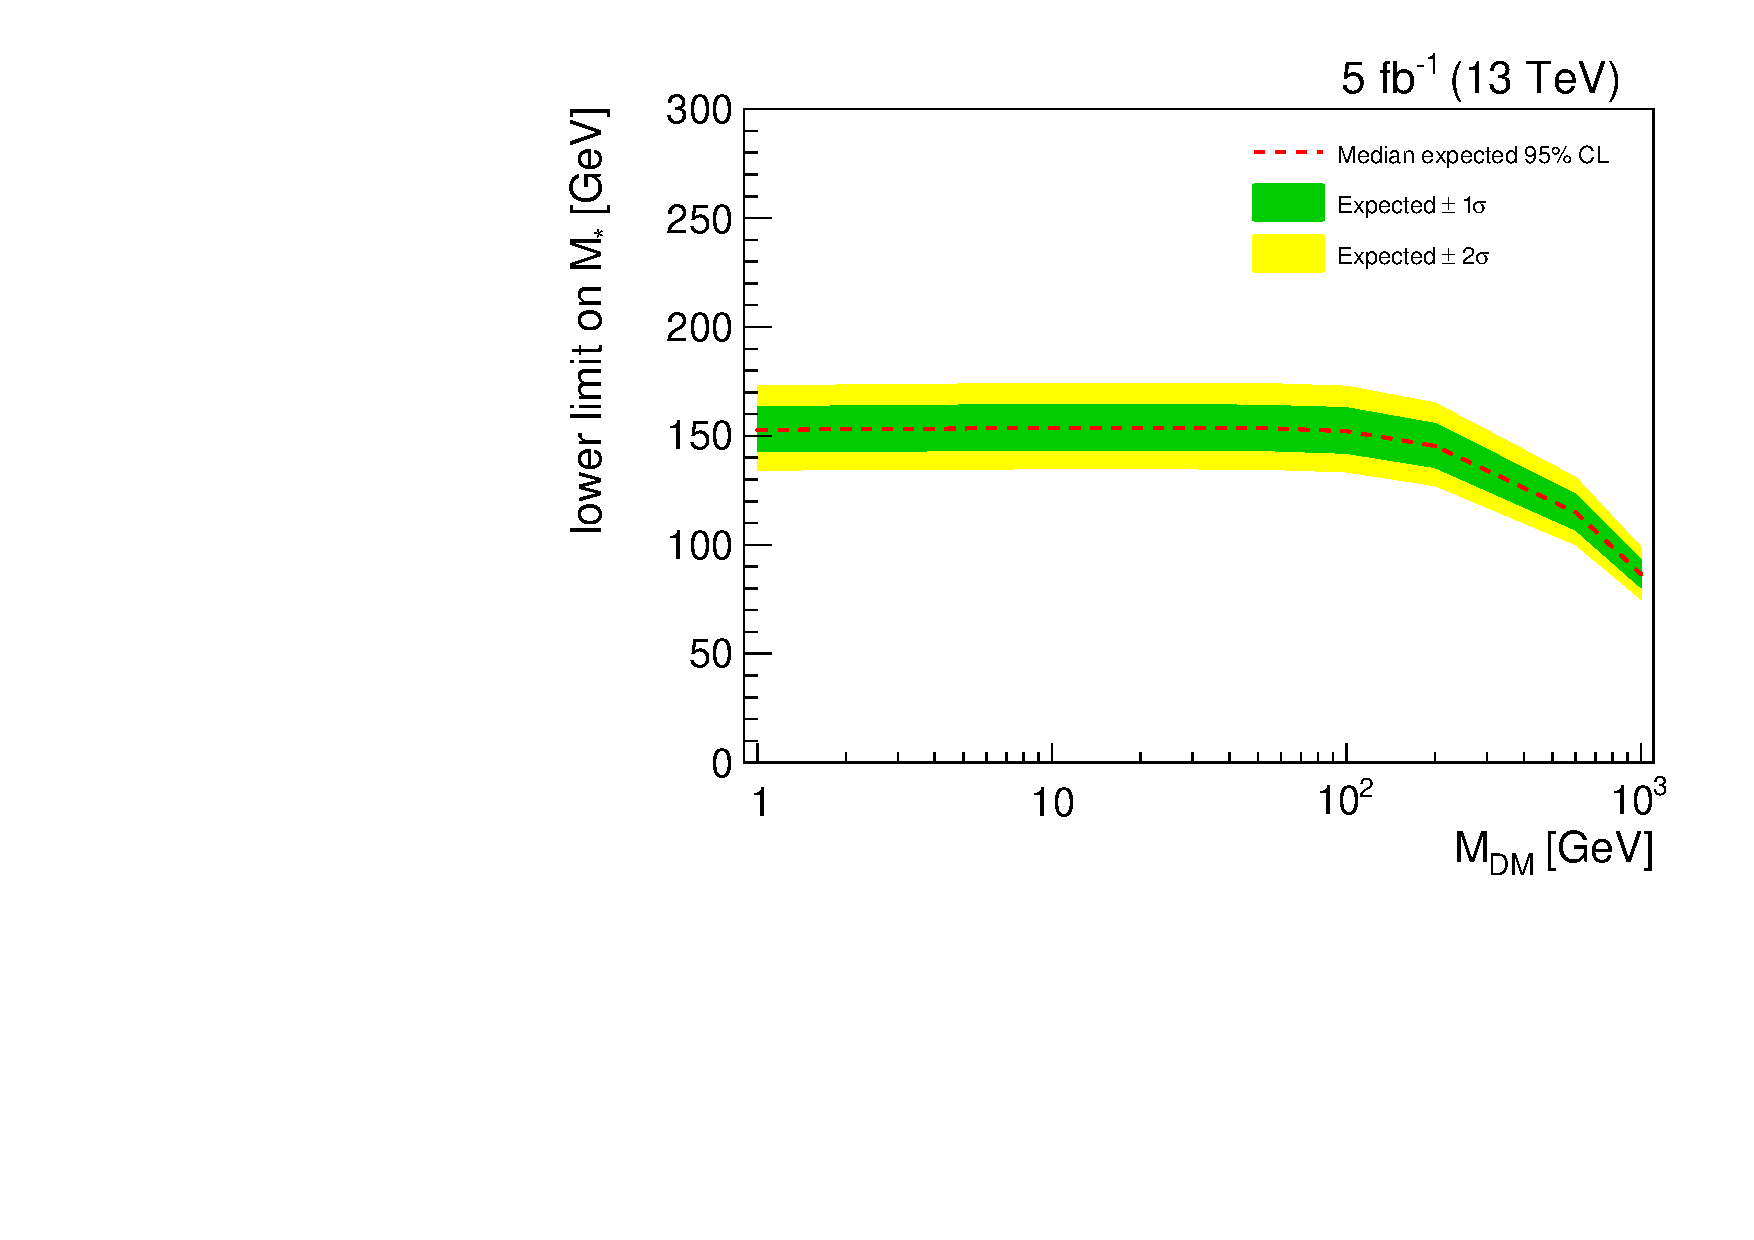
\includegraphics[width=0.32\textwidth]{figures/mstarLimit_semilept_combo_shape.pdf}}
  \subfigure[Combined]{\label{subfig:combined_cat_shapem}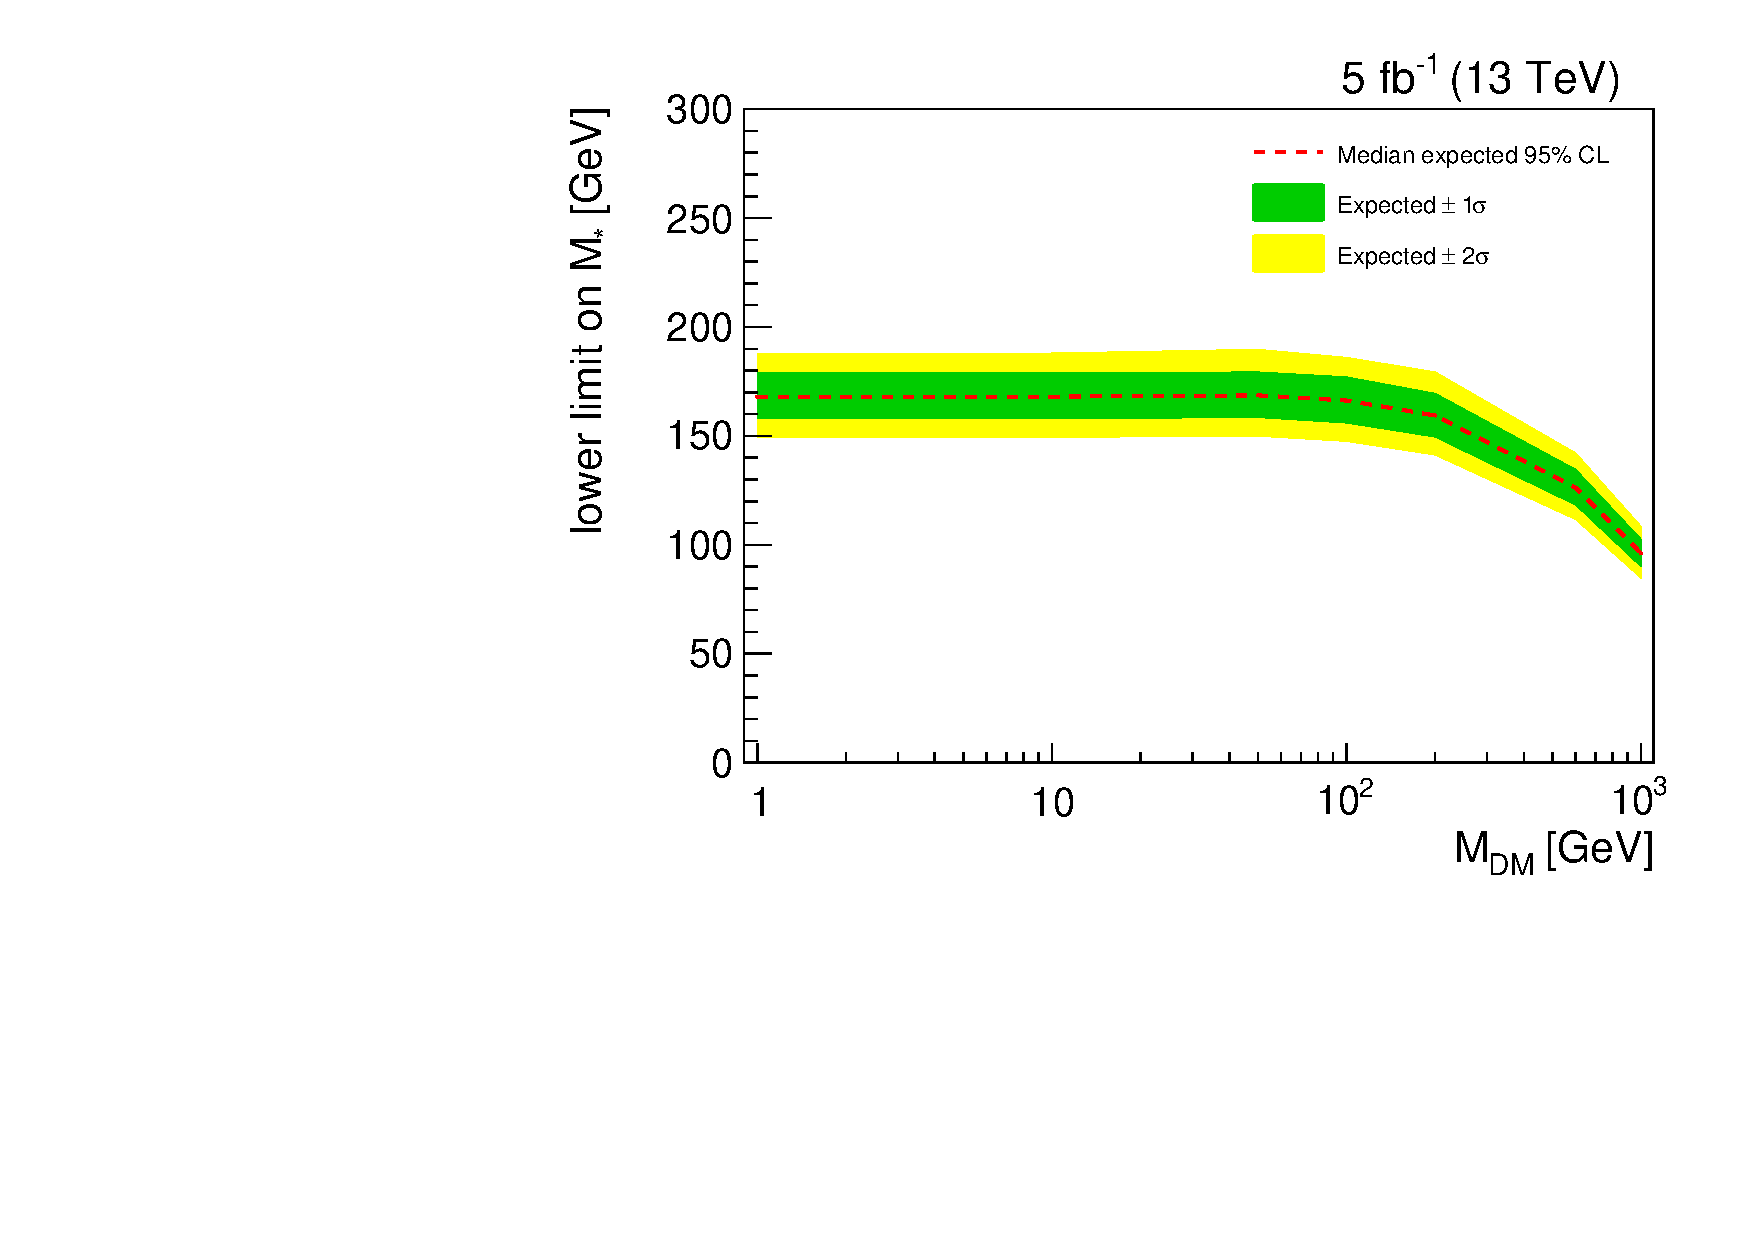
\includegraphics[width=0.32\textwidth]{figures/mstarLimit_combo_shape.pdf}}
  \caption{Expected lower limits on $M_*$ from combining all top tagging categories: \subref{subfig:hadronic_cat_shapem} hadronic channel, \subref{subfig:semilept_cat_shapem} semileptonic channel, and \subref{subfig:combined_cat_shapem} combination of both channels.}
  \label{fig:mstarlimits_combo_shape}
\end{center}
\end{figure}
